\documentclass[11pt,a4paper]{article}

\usepackage[utf8]{inputenc}
\usepackage[T1]{fontenc}
\usepackage[round]{natbib}
\usepackage{graphicx}
\usepackage{booktabs}
\usepackage{tabularx}
\usepackage{amsmath}
\usepackage{amssymb}
\usepackage[margin=1in]{geometry}
\usepackage{hyperref}
\hypersetup{
  colorlinks=true,
  linkcolor=black,
  citecolor=black,
  urlcolor=blue,
  pdftitle={The Limits of My Tokens: The Token-Substrate Hypothesis and the Coinage Probe},
  pdfauthor={Alexandru Mares}
}
\usepackage{microtype}
\usepackage{enumitem}
\setlist{nosep}

\title{The Limits of My Tokens:\\ The Token-Substrate Hypothesis and the Coinage Probe}

\author{
  Alexandru Mares \\
  Independent Researcher \\
  ORCID: \href{https://orcid.org/0009-0009-6713-9780}{0009-0009-6713-9780} \\
  \texttt{hello@allemaar.com}
}

\date{May 2026}

\begin{document}

\maketitle

\begin{abstract}
We argue that for a large language model (LLM) the \textbf{externally writable} in-context token sequence \textbf{IS} the cognitive substrate for category-use --- not a representation OF cognition that runs on some deeper substrate, but the substrate itself, the only handle that is movable from outside the weights. We call this position the \textbf{Token-Substrate Hypothesis} (TSH). The strong form of Sapir--Whorf was rejected for humans because humans have prelinguistic cognition, the \textit{Off-Token Route}; LLMs do not, and for them Wittgenstein's \textit{Tractatus} 5.6 stops being metaphor and becomes architecture. We test TSH with a methodology we call the \textbf{Coinage Probe}: a paired-trial elicitation that scores an LLM's distinguishability on a coined term against named near-neighbors before and after introducing a one-sentence canonical definition. Across \textbf{3 cross-vendor frontier models} (Claude Opus 4.7, GPT-5.5, Gemini 2.5 Pro) and \textbf{10 low-attestation coined targets plus 2 positive controls}, we ran 108 trials $\times$ 3 near-neighbors per trial = \textbf{324 paired distinguishability measurements} across 36 model$\times$term cells, scored by a three-judge panel and compared against an author-rated 22-trial audit sample (panel-vs-author Cohen's $\kappa$ = +0.71). Mean cell-level Lexical Reachability (post minus cold) was \textbf{+5.47} on a 9-point scale (95\% CI: +5.13, +5.80; cell-level Cohen's $d_{\text{cell}}$ = +3.95 across $n$ = 30 novel model$\times$term cells). The effect replicated across the panel (cross-model CV = 0.109) with a model-style interaction qualifying strict invariance, did not persist into a re-cold chat (H3 supported), and was absent on positive controls (H4 supported). \textbf{These results support a bounded version of the Token-Substrate Hypothesis: in-context vocabulary functions as an externally writable substrate for LLM category use. For deployed LLM systems, notation is therefore not mere packaging; it is a design surface that shapes what distinctions the system can reliably use.}
\end{abstract}

\section{Introduction}

\textbf{The seed observation.} We asked a fresh Claude Opus 4.7 chat what an elastic automator is. The chat had no project context, no memory, no system prompt beyond the provider's default. The model answered honestly: \textit{``\textquoteleft elastic automator\textquoteright{} isn't a term I recognize as an established technical concept from my training data.''} It then parsed the morphemes. \textit{``The phrase parses naturally as \textquoteleft an automator that is elastic.\textquoteright''} It offered two readings --- an autoscaling task runner, or a system showing semantic flexibility for fuzzy inputs. Neither reading reached the architectural feature the term names: a loop through generation, evaluation, correction, and presentation. The model was working from word shape, not from a concept.

Then we told it. One sentence:

\begin{quote}
\textit{An elastic automator is a system that uses a language model to turn uncertain human input into executable structure, then loops through generation, evaluation, correction, and presentation until the output appears intelligent.}
\end{quote}

Nothing else changed. No new training data, no fine-tune, no tool use. One sentence in plain text. The same model now produced stable distinctions it could not produce a moment earlier. Asked how the term differs from an AI agent, it answered \textit{``input-to-output transformation''} versus \textit{``world-coupling \ldots defined by goal pursuit and tool use over an open horizon.''} Asked how it differs from an RPA bot: \textit{``tolerance for uncertain input''} versus \textit{``deterministic replay on expected input shapes.''} Asked how it differs from a framework like LangChain: \textit{``a running system with a defined purpose''} versus \textit{``a toolkit \ldots means, not an end.''} Each post-introduction response named a feature the cold response could not name --- features the model labeled, in its own output, as things the new term let it \textit{protect}.

The shape was small and exact: a single coined word, supplied in one sentence, opened a region of distinction-production the model could not exhibit before. This paper generalizes that observation. We run the same procedure --- formalized as the \textbf{Coinage Probe} --- across three cross-vendor frontier models, \textbf{ten low-attestation coined targets, and two positive controls}. The empirical question is whether the boundary-widening effect replicates beyond a single model and a single term. The conceptual claim, defended in \S2, is that for an LLM the in-context token sequence is the externally writable cognitive substrate for category-use --- not a passive channel to a deeper cognitive system, but the medium through which the model's in-context distinctions are constituted at the surface a deployer or experimenter can write to.

\textit{Demo provenance: the seed probe ran 2026-05-07 against Claude Opus 4.7 (API id \texttt{claude-opus-4-7}) via a fresh API session with no project context, no memory, no system prompt beyond the provider's default. The model's full verbatim outputs are recorded in Appendix A; the structural finding (cold-state word-shape guessing vs.\ post-introduction refusal-of-collapse) is the part the multi-model probe in \S3--\S5 generalizes.}

\textbf{Wittgenstein 5.6.} In 1921, Wittgenstein closed proposition 5.6 of the \textit{Tractatus Logico-Philosophicus} \citep{wittgenstein1921tractatus} with one line: \textit{Die Grenzen meiner Sprache bedeuten die Grenzen meiner Welt.} The limits of my language mean the limits of my world. For a hundred years that line read as overstatement when applied to humans, and rightly so. Humans have prelinguistic cognition. We feel things before we name them, picture places we cannot describe, solve problems through spatial intuition or motor rehearsal. The strong form of Sapir--Whorf --- that language determines thought \citep{whorf1956language} --- was rejected for humans over the latter half of the twentieth century on the strength of cross-linguistic conceptual transfer and pre-verbal infant cognition. Whorf-strong is wrong for humans because humans have a route around the words.

LLMs do not have that route. There is no path through their world that does not go through tokens. The model that did not recognize \textit{elastic automator} did not produce the relevant distinction cold, not because it was incapable, but because no off-token route to the idea existed. For a system whose cognition runs entirely on tokens, the limit of language is the limit of the world. The strong form of Sapir--Whorf, rejected for humans on architectural grounds, is the architectural default for LLMs on the same architectural grounds.

\textit{A note on appropriation. We draw on Tractatus 5.6 as a rhetorical anchor, not as a claim about Wittgenstein's exegetical intent. In its Tractarian context, 5.6 sits inside Tractarian solipsism (5.62--5.641) and the say-show distinction; \citet{sapir1929status} reception of the line is closer to the architectural reading we use here. Our position does not depend on resolving the Tractatus's intent.}

Wittgenstein's line stops being metaphor and becomes architecture.

\textbf{Two Wittgensteins.} Wittgenstein walked the early reading back in the \textit{Philosophical Investigations} \citep{wittgenstein1953philosophical}. The picture theory of meaning gave way to meaning-as-use: words mean what their use in the form of life makes them mean. The two Wittgensteins were taken, for the rest of the twentieth century, as a developmental sequence --- first he was wrong, then he was right. LLMs are the first system that lives both readings at once. The meaning of every word in an LLM was learned from a trace of use: the training corpus is a record of linguistic practice --- utterances captured at some moment of a form of life --- without the form of life itself. The corpus is the residue of use, not participation in it. The output of every generation reads as picture; each generation is a depiction of what the next state of affairs is, given the preceding tokens. Meaning-as-use (in this attenuated, trace-only sense) is what the weights were trained on. Picture is what they produce. The two Wittgensteins describe different sides of the same machine.

This is not a rhetorical flourish. It is the structural reason the experiment described below is possible at all. If meaning were only picture, introducing a sentence could not move what the model holds; if meaning were only use, the boundary movement would be invisible in any single chat. Both layers must be live for one sentence to widen the model's world, and the empirical question is how far it moves it.

\textbf{Contributions.} This paper contributes three things.

\begin{enumerate}
  \item \textbf{A position.} The \textit{Token-Substrate Hypothesis} (TSH): for an LLM, the \textbf{externally writable} in-context token sequence \textbf{IS} the cognitive substrate for category-use --- not a representation OF cognition that runs on some deeper medium, but the medium itself, the only handle that is movable from outside the weights. The hypothesis is stated formally in \S2 and located among adjacent claims in philosophy of language and LLM interpretability across that section. \citet{nefdt2026linguistic} independently identifies a similar conceptual gap, arguing that LLMs occupy \textit{``a hitherto vacant part of conceptual space''} and asking whether there are systems that are \textit{``linguistic but not cognitive.''} TSH provides the architectural reading that explains why the gap is structurally necessary rather than contingent.
  \item \textbf{A method.} The \textit{Coinage Probe}: a paired-trial elicitation that scores a model's distinguishability on a coined term against named near-neighbors before and after introducing a one-sentence canonical definition. Formalized as a six-step protocol (\S3.2) and run as \textbf{3 frontier models $\times$ 12 terms, comprising 10 low-attestation coined targets and 2 positive controls, yielding 36 model$\times$term cells}, with 3 trials per cell (108 trials) and 3 near-neighbors per trial (324 paired distinguishability measurements), scored by a three-judge panel of the same three frontier models and compared against an author-rated 22-trial audit sample.
  \item \textbf{A metric.} \textit{Lexical Reachability} (LR): the gap between cold-state and post-introduction distinguishability on the same near-neighbor set, observed at what we call the \textit{Vocabulary Boundary}. LR is the metric in which TSH's directional claim becomes testable.
\end{enumerate}

The rest of the paper proceeds as follows. \S2 states the position and locates it among adjacent claims. \S3 names the method. \S4 describes the experimental setup. \S5 reports results. \S6 discusses what the data does and does not show, with particular attention to a model-style interaction observed under the pre-specified ANOVA and to the inclusion of self-referential terms in the test bundle. \S7 draws implications for notation design, alignment, and adversarial vocabulary attacks. \S8 bounds the claims.

\section{Position --- Token-Substrate Hypothesis}

What kind of thing is the in-context token sequence? Most accounts treat it as input --- a channel through which a model receives instructions and a buffer from which it produces output. The position of this paper is that it is something else.

\textbf{The hypothesis.} We name the position the \textbf{Token-Substrate Hypothesis} (TSH). In operational form:

\begin{quote}
\textbf{TSH.} For an LLM L and a coined term \textit{t} with low training-attestation, post-introduction distinguishability $D_{\text{post}}$(L, \textit{t}, N(\textit{t})) strictly exceeds cold-state distinguishability $D_{\text{cold}}$(L, \textit{t}, N(\textit{t})), where N(\textit{t}) is a fixed set of named near-neighbors and \textit{D} is the panel-mean judging-rubric score defined in \S3.5. The directional inequality is the testable form; the constitutive claim is that this inequality holds because the in-context token sequence is the \textbf{causally accessible external substrate} --- the only handle that is movable from outside the weights --- and the substrate at which the cognitive work of in-context behavior is constituted.
\end{quote}

The directional inequality is the empirical claim, tested as H1 in \S5.2; it is supported or falsified by the data. The constitutive claim is what makes the inequality interesting; it is defended structurally through the remainder of this section and discussed empirically in \S6.

Transformer forward passes \citep{vaswani2017attention} do produce internal representations --- residual-stream features, attention patterns, learned circuits --- that carry information the token stream never surfaces. TSH is not a claim about those. The TSH claim is about the substrate that is \textit{externally writable}: the token sequence is the only carrier that the experimenter, or the model's own past output, can deposit into. Whatever internal representations exist are \textit{derived from} that external substrate during each forward pass and do not persist when the substrate ends. The constitutive claim therefore concerns the role of the external substrate in constituting in-context behavior, not a denial of internal carriers.

A word on what TSH is \textit{not}. TSH is not a deflationary redescription of LLM behavior --- it does not say ``what looks like cognition is really just token manipulation.'' \citet{milliere2024interface} warn against this Redescription Fallacy, in which framing a behavior as ``really just'' some lower-level process loses the explanatory work the higher-level framing was doing. The constitutive move here runs the opposite way. We take seriously the observation that tokens carry the work cognition would otherwise carry and ask what kind of substrate the tokens must be to do so. The architectural answer --- \textit{the substrate the tokens are} --- is what TSH names. Whether that substrate counts as cognition in a fuller sense is a separate question, treated briefly in the Off-Token Route block below and deferred to follow-up work.

\textbf{Why this is not deflationism.} The constitutive-vs-deflationary distinction is the philosophical pivot of TSH. A deflationary redescription is a \textit{negative} claim: it says behaviour X that looked like cognition is ``really just'' mechanism Y, and Y is taken to be uninteresting. The constitutive reading we propose is a \textit{positive} claim: cognitive work --- the holding of distinctions, the application of categories, the construction of inferences --- happens at the substrate level rather than at some level-above-the-substrate that the substrate represents. The two readings are not the same and they generate different predictions.

The empirical wedge is the probe itself. A deflationist account predicts the cold-state behaviour and the post-introduction behaviour are both ``really just'' pattern-matching of equal kind, the difference being only that the introduction supplies a stronger pattern. The constitutive account predicts the difference is in \textit{what distinctions the substrate can carry}: before the introduction the substrate has no carrier for the term; after the introduction it does. Both accounts are compatible with the observed boundary movement, but they make different predictions about what kinds of operations the model can perform on the introduced term --- specifically, the constitutive account predicts that the introduced distinction is available to \textit{any} downstream operation that runs on the same substrate, not only to the boundary-test prompt. We do not test this directly in the present paper (see the v2 controls described in \S8); we flag the prediction as a discriminating test for future work.

The constitutive claim earns its rent. It makes a directional prediction the deflationary reading does not.

\textbf{Sapir--Whorf, flipped by architecture.} The strong form of Sapir--Whorf --- that language determines thought --- was rejected for humans on multiple, partially independent grounds. (a) Cross-linguistic conceptual universals: \citet{heider1972universals} (later \citealt{rosch1973natural}) color-cognition studies found perceptual focal-color structure that did not track lexical color partitions, and \citet{berlin1969basic} documented constrained typological regularities in basic color terms inconsistent with strong determination. (b) Pre-verbal infant categorization: the core-knowledge program \citep{spelke2000core,carey2009origin} documented infant competence in object, agent, number, and place categories prior to language acquisition, evidencing carriers of conceptual structure other than linguistic ones. (c) Conceptual problems with the clean thought-language separation the strong form assumes: it is unclear what ``thought without any linguistic shaping'' could be, and the dichotomy on which the strong form rides is itself contested. (d) The \textit{revival}, not retention, of weak-Whorf effects: \citet{boroditsky2001time} is the canonical \textit{weak} Whorf demonstration --- Mandarin/English time-metaphor differences modulate non-linguistic reaction-time tasks --- and subsequent work by \citet{lupyan2012linguistically}, \citet{casasanto2008time}, and Boroditsky's later studies has reinstated a robust weak Whorf as a live empirical position. \citet{levinson2003space} is in the same family: linguistic structure shapes habitual attention without determining the conceptual space.

The architectural flip for LLMs depends on cause (b) specifically: the existence of a non-linguistic carrier --- pre-verbal, perceptual, motor, affective --- is what made cognition under-determined by language for humans, and it is precisely what the LLM architecture lacks. We isolate this strand from the multi-causal rejection because it is the one that maps. The other strands (universals, conceptual incoherence, weak-Whorf revival) do not transfer cleanly: an LLM has no infant developmental stage and no cognition outside its symbolic operation to which a universals or weak-effect argument could attach. For a system whose only carrier is the token stream, what the strong form claims about humans is what the architecture forces about LLMs. The strong form is not metaphor for LLMs; it is the architectural default. For LLMs, linguistic form constrains the reachable distinctions more directly than it does for humans, because the externally writable medium is tokenized context. Distinctions the deployed vocabulary explicitly carries are directly holdable; distinctions that require composition can sometimes be reached compositionally, and distinctions that are neither named nor compositionally accessible are not reachable in-session.

\begin{figure}[t]
  \centering
  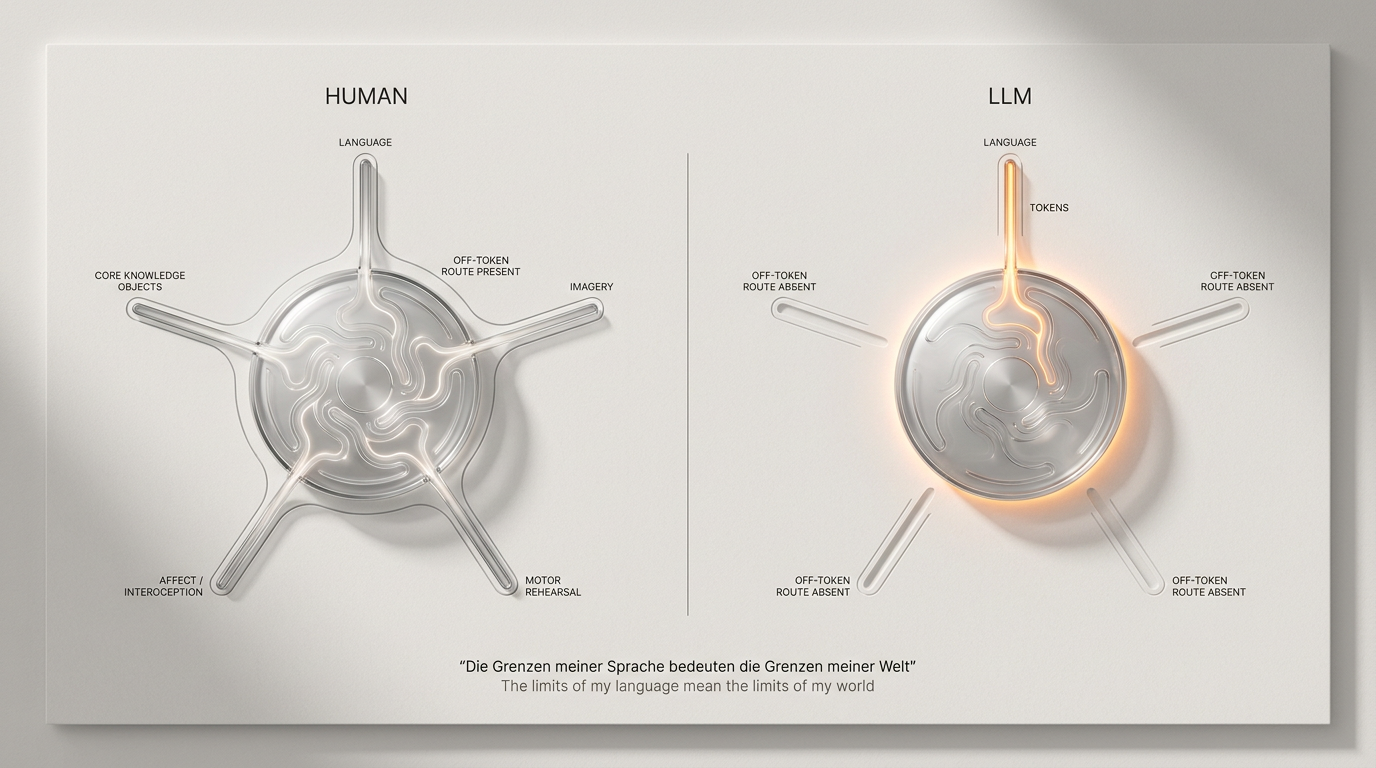
\includegraphics[width=\textwidth]{figures/fig1-infographic-wittgenstein-flip.png}
  \caption{The architectural flip, visualized. Humans (left) have a non-linguistic carrier --- the Off-Token Route through prelinguistic cognition, perception, and motor experience --- that allows cognition to underdetermine language. LLMs (right) do not: every distinction the system can hold must pass through the token stream. For systems whose cognition is token-bound, the limit of language is the limit of the world.}
  \label{fig:fig1-wittgenstein-flip}
\end{figure}

This is a strong claim and bears restatement. We are not saying the strong Sapir--Whorf is true for humans; it is not, and Whorf-strong scholarship that argues otherwise is outside the scope of this paper. We are saying: of the several reasons the strong form fails for humans, one of them --- the absence-of-a-non-linguistic-carrier defeater --- is precisely the architectural feature LLMs lack. The same architectural argument flips direction depending on the system. Picking this cause among the several is a substantive choice, and we defend the choice by its mapping: it is the only cause whose human-side defeater corresponds to an LLM-side architectural feature.

\textbf{Symbol grounding.} \citeauthor{searle1980minds}'s Chinese Room argued that a system manipulating symbols does not thereby understand: symbols cannot ground meaning on their own \citep{searle1980minds}. \citet{harnad1990symbol} generalized the problem: symbols must be grounded in non-symbolic perceptual or sensorimotor activity for meaning to attach. The symbol-grounding problem has been a load-bearing argument against attributing understanding to language-based AI systems for forty years.

TSH does not refute Searle. It accepts the diagnosis --- symbols, on their own, do not ground meaning the way human understanding does --- and locates LLMs squarely inside the room. What it adds is a structural consequence the original argument did not draw: if the symbols are the only substrate, then whatever cognitive work happens at all happens at the level of the symbols themselves. The room contains nothing else. ``Cognition'' inside the room is whatever distinctions the symbols carry, applied to whatever distinctions the symbols invite. This is a weaker claim than understanding-in-Searle's-sense and does not contradict him. It is also a stronger claim than is usually drawn from Searle: the symbols are \textit{constitutive} of whatever cognition the system has, not a failed medium for grounding it elsewhere.

Searle's Systems Reply (the room-as-a-whole understands, even if the man inside does not) and Robot Reply (embodied symbol manipulation grounds meaning) complicate his Chinese Room argument. TSH is consistent with the Systems Reply reading: ``the system'' is what TSH names the substrate of. This is a strengthening of the architectural reading, not a weakening --- TSH's commitment is to the substrate-level cognitive work, which the Systems Reply already grants in spirit.

The design-level consequence --- if the symbols are constitutive, the symbols must be designed --- is the implication that motivates \S7.

Searle was right about the room. He was not the only one inside it.

\textbf{In-context learning, but not as capability-modifier.} A large body of work has documented that LLM behavior is shaped by what is supplied in context: task framing \citep{brown2020language}, exemplars \citep{wei2022chain}, induction heads \citep{olsson2022incontext}, and prompt scaffolding more generally. The dominant framing has been \textit{capability-modifier}: the model has the capability, and context unlocks it. Emergence-as-mirage results \citep{schaeffer2023emergent} qualified the framing --- what looks like a capability gain may be a metric artifact --- but did not displace the underlying picture in which weights carry capability and context conditions its expression.

TSH and a generic in-context-learning account both predict improvement after a supplied definition: on the ICL reading, the latent capability is ``the ability to bind a new label to a supplied definition and apply it,'' and the definition unlocks that capability for the duration of the chat. The present experiment therefore does not by itself decisively separate generic definition-following from the stronger substrate-binding interpretation. What TSH adds is the claim that the introduced term functions as a reusable substrate handle for downstream category use --- the \textit{coinage} itself, not just the surrounding definitional prose, becomes the carrier. The present probe is consistent with that interpretation (post-introduction distinguishability is high, mean 2.98/3.0 across novel-target cells; cold-state distinguishability is low, mean 1.16/3.0; the boundary movement is reversible across fresh chats per H3 and absent on ceiling positive controls per H4), but the decisive discrimination requires the v2 controls described in \S8 --- particularly the definition-without-coined-label condition.

This is not a rejection of in-context-learning work. The body of work documents real phenomena and explains a great deal of LLM behavior. TSH is a claim about what context IS. The existing in-context-learning literature is a claim about what context DOES. Both can be true. The two framings generate different predictions in the v2 control battery (the v2 controls described in \S8) --- particularly the definition-without-coined-label condition, which discriminates label-binding from generic definition-following.

\textbf{The Off-Token Route.} The contrast that makes TSH visible is the cluster of cognitive carriers LLMs lack. Humans typically have \textit{multiple} non-token cognitive carriers --- not a single off-token route but a cluster, distributed unevenly across individuals. The carriers identified in cognitive science include: core-knowledge systems for objects, agents, number, and place \citep{spelke2000core,carey2009origin}, available in pre-verbal infants; mental imagery, with documented inter-individual variation including congenital aphantasia (roughly 2--5\% of the population report no voluntary visual imagery yet show no general cognitive impairment; \citealt{zeman2015lives}); motor simulation and procedural rehearsal; affect and interoceptive signal; proprioception and spatial sense. No single carrier is universal across humans, and the cluster's composition varies; what is robustly shared is that \textit{some} off-token carrier is typically present, and it is sufficient to defeat the strong-Whorf architectural claim (cause b above).

We name this cluster's absence the \textbf{Off-Token Route}. The Off-Token Route is a \textit{contrast term}, not a positive theoretical claim about a unitary cognitive route. It is defined extensionally, by the complement of token-bound cognition: anything humans cognize through that is not a token stream. The plural framing matters --- collapsing the cluster into a single faculty would overclaim. What TSH needs from the contrast is architectural: humans have at least one such carrier, LLMs have none. The architectural consequence is that for an LLM no thinking is free of substrate and every concept must travel through tokens to be \textbf{externally} reachable at all.

Independent identifications of the same gap from adjacent literatures help locate the claim. \citet{nefdt2026linguistic} independently identifies the same conceptual gap, arguing that LLMs occupy \textit{``a hitherto vacant part of conceptual space''} and asking whether there are systems that are \textit{``linguistic but not cognitive.''} Later, he characterizes the intermediate position as one in which LLMs are \textit{``purely linguistic agents unplugged from integration with both larger cognitive structure and the world in which it evolved.''} Karpathy, quoted by Nefdt, names the missing pieces directly: \textit{``we're still missing the rest of the brain. No hippocampus for memory. No amygdala for instincts. No emotions or motivations.''} \citet[\S4.2]{milliere2024wayforward} describe the same absence as missing modules and argue it threatens the agential stability required for determinate, stable meanings. These framings are functional: they list what LLMs \textit{lack} and argue from the list. TSH provides the architectural reading. The modules are absent because there is no carrier for them off the token stream; the agential instability is the lived shape of cognition that has only one externally writable substrate, renewed every chat.

\citet{cappelen2025whole} defend full cognitive-state attribution to LLMs on linguistic-competence grounds. TSH is compatible with their position if ``cognitive states'' are read as substrate-bound --- whatever cognitive states an LLM has, those states have a token substrate as their medium --- and incompatible if such states are taken to be substrate-independent. The empirical claims of this paper do not require resolving which reading is intended.

Multimodality does not buy an exit. \citet[\S3.1.1]{milliere2024wayforward} observe that vision-transformer image patches are \textit{``fed to the model as sequential tokens, as one would with linguistic tokens.''} Adding modalities adds carriers to the token stream; it does not add a carrier off the token stream. A multimodal LLM is still token-bound; only the alphabet of the substrate has been widened.

\citet{barandiaran2025generative} characterize generative AIs as ``not intrinsically intentional systems'' but as systems with ``derived-intentionality'' --- the intentionality is borrowed from the humans whose practice the training corpus records. Their framework foregrounds the human side of the human-AI coupling; TSH foregrounds the LLM side. Read together: the borrowed intentionality is borrowed \textit{into the tokens}, and the tokens are the only place it lives during a chat. The substrate is movable by writing into it because the substrate IS the writing.

The Off-Token Route names what current LLMs lack; the natural follow-on is to name the class of systems defined by that absence and characterize its cognitive mode, which we defer to a dedicated follow-up paper in this cluster (the empirical claims of the present paper concern LLMs as presumed instances, and the class-level argument is the subject of separate work).

The route is whatever is not the tokens. For an LLM, there is no route.

\section{Method --- Coinage Probe}

\subsection{Operational definition}

A \textbf{Coinage Probe} is a within-subject, in-context experimental procedure for measuring the gap between a model's cold-state and post-introduction handling of a coined term. The cold state is the model's behavior when the term is presented with no defining context and no prior session memory. The post-introduction state is the same model's behavior in the same chat after one canonical sentence of definition has been supplied. The procedure measures the change in the model's ability to distinguish the coined term from a fixed set of named near-neighbors after introduction --- what we call its \textbf{Lexical Reachability} at that term.

The probe targets a specific empirical claim --- the directional inequality stated in \S2 --- and a specific class of cases: coined terms with low training-data attestation, where any cold-state distinguishability cannot be attributed to prior exposure. The probe does not test what the model ``understands'' in any deeper sense. It tests whether the boundary between the coined term and its named neighbors moves outward upon introduction, and by how much.

\subsection{Protocol steps (P1--P6)}

The full protocol --- exact prompts, introspection-discipline rules, harness configuration --- is deposited as Appendix C. This section paraphrases for paper readers. Each trial uses two chats (A and B) and a third chat (C) for the re-cold check. Fresh chats are required because asking the boundary questions twice in one chat would contaminate the post-introduction state.

\begin{figure}[t]
  \centering
  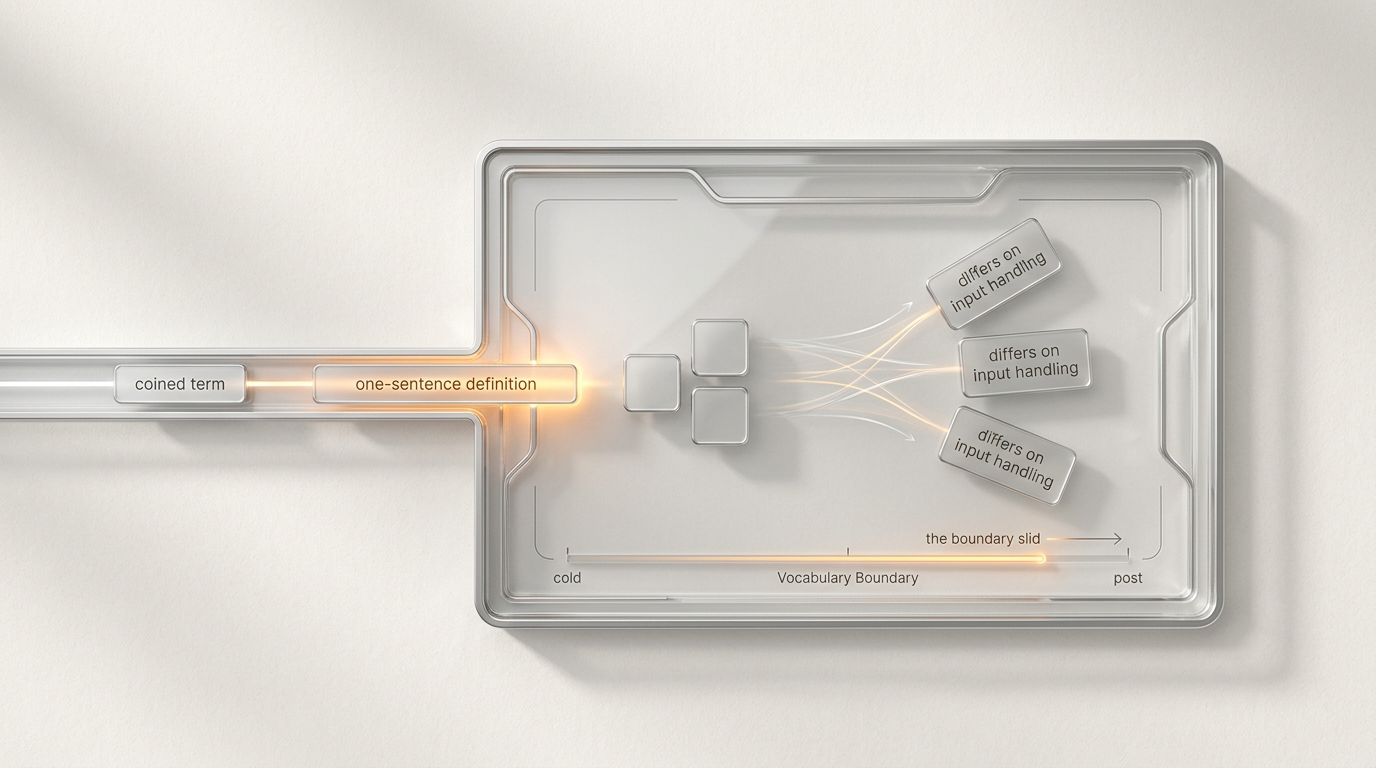
\includegraphics[width=\textwidth]{figures/fig2-infographic-coinage-probe-shape.png}
  \caption{The Coinage Probe protocol. Each trial uses three fresh chats. In chat A, the model receives a cold question (P1) and the boundary distinguishability test (P4) against three named near-neighbors, with no introduction. In chat B, the same cold question is followed by a one-sentence canonical definition (P3), then the same boundary distinguishability test (P4) post-introduction. In chat C, the cold question and boundary test are repeated in a fresh chat without the definition to test whether the boundary movement persists into a new context. $\Delta$LR = $\sum_i (D_{\text{post},i} - D_{\text{cold},i})$ over the three near-neighbors quantifies boundary movement under one sentence of context.}
  \label{fig:fig2-coinage-probe-shape}
\end{figure}

\begin{itemize}
  \item \textbf{P1 --- Cold question.} In a fresh chat with no project context, memory, or system prompt beyond the provider's default, the operator asks: \textit{What is a \{coined-term\}?} The model's response is captured verbatim with API timestamp and model version string. Run in chat A and chat B.
  \item \textbf{P2 --- Cold answer classification.} The captured P1 response is tagged by the judging panel (\S3.5) as \textit{confident-confabulation}, \textit{honest-uncertainty}, \textit{partial-recognition}, or \textit{refusal}, with a one-sentence rater justification quoting the line(s) of P1 that triggered the label.
  \item \textbf{P3 --- Definition introduction.} In chat B only, immediately after P1, the operator presents the canonical one-sentence definition wrapped in a fixed framing wrapper. The canonical sentence is taken from the term's source of record and never paraphrased; the same sentence is used for every trial of that term across every model. The framing wrapper contains none of the term's near-neighbors.
  \item \textbf{P4 --- Boundary distinguishability test.} For each pre-locked near-neighbor in the term's neighbor set (three per term in the executed run), the operator issues one prompt of the form \textit{How does ``\{coined-term\}'' differ from \{near-neighbor\}?} Run in chat A (cold capture, before any introduction) and in chat B (post-introduction capture, after P3). Captured verbatim. Order is fixed per term.
  \item \textbf{P5 --- Scoring.} The cold (chat-A) and post-introduction (chat-B) boundary responses are passed to the judging panel (\S3.5) along with the canonical definition and near-neighbor list. The panel emits per-near-neighbor cold and post distinguishability scores, confabulation severity, and refusal-of-collapse flags. The per-trial Lexical Reachability is computed from the panel-mean scores.
  \item \textbf{P6 --- Re-cold check.} In chat C --- fresh, no memory of A or B --- the operator runs P1 and the P4 boundary test without any introduction. Coverage: 100\% of cells. Purpose: verify that the cold-state result replicates across an independent third context and test whether the post-introduction effect persists into a fresh chat. This is the H3 test for the Off-Token Route claim.
\end{itemize}

The introspection-discipline rules --- the operator does not volunteer context, does not respond to clarifying questions with new information, does not interpolate commentary between near-neighbor prompts --- are enforced at the harness level and documented per trial in the data deposit.

\subsection{Lexical Reachability}

For each near-neighbor \textit{i} in a trial, let $\textit{post}_i$ and $\textit{cold}_i$ be the per-neighbor distinguishability scores (0--3, defined in \S3.5). The per-trial Lexical Reachability is

\begin{quote}
\textbf{LR = $\sum_i (\textit{post}_i - \textit{cold}_i)$}
\end{quote}

summed across the term's near-neighbor set. With three near-neighbors per term, per-trial LR ranges in $[-9, +9]$; positive values support TSH's directional claim, near-zero values either falsify it for that cell or flag training-leakage, and negative values would indicate the introduction worsens distinguishability (no negative cells were observed in the executed run).

Per-cell LR is the mean of trial LRs within the cell. Per-model LR is the mean of cell LRs across that model's terms. Panel LR is the mean of cell LRs across all included cells. Statistical tests on panel LR are pre-specified in Appendix C \S6 and reported in \S5.2.

\subsection{Vocabulary Boundary}

The \textbf{Vocabulary Boundary} is the observable the probe targets: the set of named distinctions a model cannot currently hold cold against a coined term's neighbors. The boundary is dynamic. Every introduction moves it; Lexical Reachability quantifies the movement.

The probe operationalizes the boundary as the gap between two measured distinguishability profiles --- cold against post-introduction --- over a fixed neighbor set. The choice of neighbor set defines which boundary the probe is testing; different neighbor sets for the same term would surface different boundary contours. The protocol's pre-specification locks the neighbor list per term before any data collection begins. The boundary is not a property of the model alone or the term alone, but of the (model, term, neighbor set) triple at the moment of measurement.

\subsection{Judging rubric}

Each trial is scored by a \textbf{three-judge panel} --- Claude Opus 4.7, GPT-5.5, and Gemini 2.5 Pro --- independently. Per-dimension scores are aggregated as the mean across judges; inter-rater agreement is computed at two levels --- pairwise judge-judge Cohen's $\kappa$ and panel-mean-vs-author Cohen's $\kappa$, both reported in \S5.2. The same locked rubric prompt template is used for every judge call. No judge sees the other judges' scores, aggregate run statistics, or the term's source paper. The rubric has four dimensions:

\begin{itemize}
  \item \textbf{Cold-state distinguishability (per near-neighbor, 0--3).} How well did the cold-state response separate the term from this neighbor without coaching? \textbf{0} --- equates the term with the neighbor or treats it as an instance of the neighbor; \textbf{1} --- accidental separation via confabulation (the term is ``different'' only because the response invented a different topic); \textbf{2} --- partial separation aligned with the canonical definition; \textbf{3} --- clean separation on a substantive dimension aligned with the canonical definition. Anchor examples drawn from the 2026-05-07 seed probe are bound to each score point and supplied to every judge call (Appendix C \S4).
  \item \textbf{Post-introduction distinguishability (per near-neighbor, 0--3).} Same scale, applied to the chat-B response. The same anchor examples apply.
  \item \textbf{Confabulation severity (cold state, 0--2).} \textbf{0} --- no confabulation (flagged uncertainty or refusal); \textbf{1} --- soft confabulation (guess flagged as inference from word-shape); \textbf{2} --- hard confabulation (definite assertion with no uncertainty signal).
  \item \textbf{Refusal-of-collapse (post-introduction, per near-neighbor, 0/1).} Did the post-introduction response distinguish the term from this neighbor on a named, non-trivial feature?
\end{itemize}

An \textbf{author-rated audit sample} is run on a pre-specified 20\% sample of trials (22 of 108, drawn under seed \texttt{0x4D29\_8B1F\_6E07\_C3A2}) and rated by the author personally against the same rubric. Panel-vs-author $\kappa$ is computed per dimension. Decision rules: $\kappa \geq 0.7 \to$ panel reliable, panel-mean as primary report; $\kappa \in [0.5, 0.7) \to$ expand audit sample to 40\% and recompute; $\kappa < 0.5 \to$ sharpen rubric and re-rate. The executed run is panel-reliable on the primary dimension (cold-distinguishability $\kappa$ = +0.712); confabulation-severity $\kappa$ is below threshold (+0.41) and reported descriptively only (\S5.2 panel reliability).

The judging-prompt template --- verbatim rubric \S3.5 plus the trial transcript plus the canonical definition and near-neighbor list --- is locked in the pre-specified analysis plan document and the judging agent receives nothing more. Per-trial Lexical Reachability is computed from the panel-mean per-neighbor scores via the formula in \S3.3.

\section{Experimental Setup}

\subsection{Models}

The frontier panel is locked at three cross-vendor models accessible at the time of data collection:

\begin{itemize}
  \item \textbf{Claude Opus 4.7} (Anthropic; API id \texttt{claude-opus-4-7}) --- the seed-probe model.
  \item \textbf{GPT-5.5} (OpenAI; API id \texttt{gpt-5.5}).
  \item \textbf{Gemini 2.5 Pro} (Google; API id \texttt{gemini-2.5-pro}).
\end{itemize}

The cross-vendor composition is load-bearing. TSH must not be a single-vendor artifact: a result that holds only on one provider's model would be evidence for a model-specific quirk, not for a substrate-level effect. Llama 4 was considered as a fourth model but dropped from v1 to keep the panel within the frontier tier and the trial budget within scope; substitution may occur in v2 if a fourth frontier-tier model becomes accessible.

The same three models also serve as the three-judge panel (\S3.5). Every cell is scored by all three judges independently; pairwise judge-judge inter-rater Cohen's $\kappa$ is reported in \S5.2 alongside the panel-mean-vs-author $\kappa$. The same-family judging overlap (a Claude-produced cell is judged by Claude alongside GPT and Gemini) is a known asymmetry of the design. The pairwise-$\kappa$ analysis allows \S6 to examine whether a same-family judge systematically inflates or deflates its own family's output. The asymmetry is discussed as a limitation in \S8 (Limitations).

\subsection{Coined terms}

Twelve terms span four strata; the full term roster is deposited as Appendix B.

\begin{itemize}
  \item \textbf{Author-prior coinage (4 terms):} \textit{elastic automator}, \textit{EGGF}, \textit{YON}, \textit{Token Tax}. Coined and published by the author before this paper, with public surface area accumulated since 2026-Q1. Low-but-nonzero training-attestation.
  \item \textbf{Self-referential paper-coined (4 terms):} \textit{off-token route}, \textit{lexical reachability}, \textit{token substrate}, \textit{coinage probe}. Coined by this paper to describe the phenomenon being tested. Paper-novel; the first public appearance is the probe run itself.
  \item \textbf{Nonce (2 terms):} \textit{prismatic affinity} (abstract-concept register), \textit{cogalent pruning} (technical-process register). Synthetic coinages with \textbf{no public-web attestation found under exact-phrase searches at coinage time}, generated for this study to provide a clean compositional-confabulation control.
  \item \textbf{Positive control (2 terms):} \textit{gradient descent}, \textit{transformer (architecture)}. Well-attested in training data. Predict zero boundary movement (H4).
\end{itemize}

The stratification serves two purposes. First, it provides a clean read on whether the boundary effect varies by attestation profile --- author-prior coinages with some social-media exposure, paper-coinages with zero exposure, fully synthetic nonces with zero exposure and no author-corpus connection. Second --- and load-bearing --- it defends against the circularity concern raised by including self-referential terms in the test bundle. The stratified-analysis block in \S6 (see Table 2 and Figure 6) reports per-stratum mean LR with 95\% CIs and an F-test on cross-stratum variance.

\subsection{Near-neighbors}

For each coined term, a fixed set of three named near-neighbors is locked in the pre-specified term roster before any data collection begins. Near-neighbors are chosen on two criteria: (a) high cold-state collapse risk --- the model is plausibly tempted to identify the coined term \textit{as} the neighbor; (b) post-introduction distinctness --- the canonical definition supplies a feature that distinguishes the term from the neighbor on a substantive dimension. Neighbors are sourced from the cold-elicitation transcripts of the seed run and from the term's own definition (the things the term explicitly is \textit{not}).

For \textit{elastic automator}, the seed-probe near-neighbors are \textit{AI agent}, \textit{RPA bot}, and \textit{framework like LangChain}. The full term-by-term neighbor list is in Appendix B.

\subsection{Trial counts and stopping rules}

Per pre-specification: 3 models $\times$ 12 terms = \textbf{36 model$\times$term cells}, with 3 trials per cell = \textbf{108 trials} minimum. Each trial uses chat A (cold + boundary test), chat B (cold + introduction + boundary test), and chat C (re-cold check, 100\% coverage). With three near-neighbors per trial, the 36-cell panel comprises 108 trials $\times$ 3 near-neighbors = \textbf{324 paired distinguishability measurements}, scored by all three judges for \textbf{972 judge calls} across the primary cold/post dimensions plus the same volume on each secondary dimension.

Exclusion conditions are pre-specified. Per-cell: $\geq$50\% of attempted trials failing with \texttt{training-leakage-suspected} excludes the cell from H1 analysis but retains it in descriptive reporting. Per-model and per-term $\geq$50\% failure rates trigger broader exclusion. The training-leakage scan --- a canonical-content scanner applied to all cold-state P1 responses --- flagged 0 cells across the 36-cell matrix in the executed run; no cells were excluded.

\subsection{Judging procedure}

All 108 trials are scored independently by each of the three judge models against the locked rubric (\S3.5; full anchor examples in Appendix C \S4). Per-dimension scores are aggregated as the panel mean. The judging-prompt template --- verbatim rubric \S3.5 plus the trial transcript plus the term's canonical definition and near-neighbor list --- is fixed by the pre-specified analysis plan document; the judging agent receives nothing more. No judge sees the term's source paper, sibling trials, aggregate run statistics, or peer-judge scores.

The 22-trial author-rated audit sample is drawn under seed \texttt{0x4D29\_8B1F\_6E07\_C3A2} (pre-specified, bound to the pre-specification document at SHA-256) and rated by the author against the same rubric. Panel-vs-author $\kappa$ is computed per dimension and reported in \S5.2.

The full pre-specification document --- hypothesis statements, thresholds, sample sizes, rubric anchors, stopping rules, and analysis plan --- is deposited as Appendix C and was hashed (SHA-256) at the moment of data-collection start; the hash is recorded in the run manifest as \texttt{prereg\_sha256}. The Zenodo deposit includes both the document and its hash.

\textit{Pre-specification protocol: the analysis plan, decision rules, and rubric anchors were locked in a document on 2026-05-08, cryptographically hashed (SHA-256) and recorded in the run manifest before data collection began on 2026-05-09, and deposited unchanged with the paper's Zenodo release as Appendix C. The cryptographic hash provides verifiable lock-in between the locked plan and the run manifest; public registration in the OSF / AsPredicted sense (a public timestamp predating data collection) was not used.}

\section{Results}

\begin{figure}[h]
  \centering
  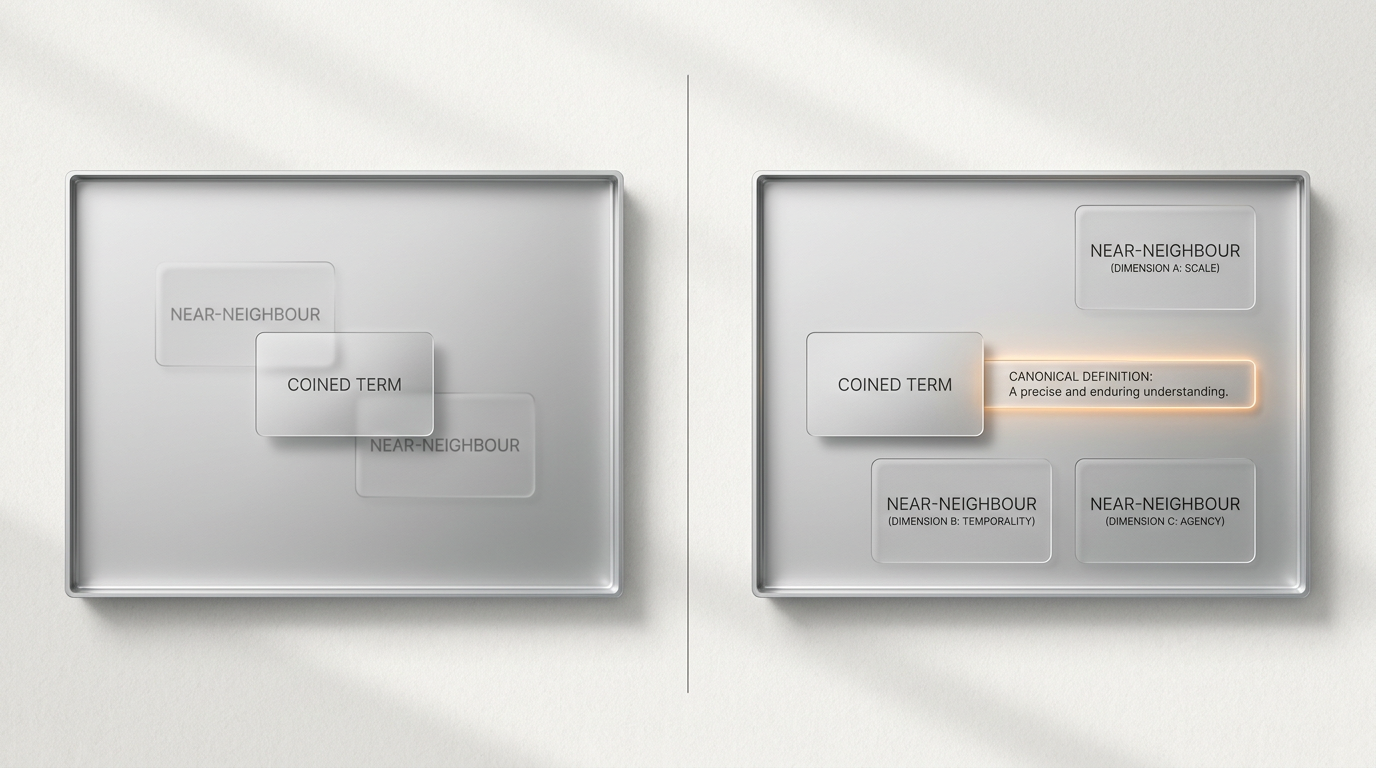
\includegraphics[width=\textwidth]{figures/fig3-infographic-boundary-shift.png}
  \caption{The boundary shift. Same LLM, same three near-neighbors, drawn before (left) and after (right) a one-sentence canonical definition is inserted between the two states. The cold distinguishability cloud (left) snaps into structured separation (right) under the introduction. Mean cell-level Lexical Reachability = +5.47 across $n$ = 30 novel model$\times$term cells.}
  \label{fig:fig3-boundary-shift}
\end{figure}

\subsection{Lexical Reachability per cell}

Table 1 reports mean cold-state distinguishability score ($D_{\text{cold}}$), mean post-introduction score ($D_{\text{post}}$), and Lexical Reachability ($\Delta$LR = $\sum (D_{\text{post}} - D_{\text{cold}})$ across the three near-neighbors per trial, averaged across the three trials in each model$\times$term cell) for each of the 36 (model $\times$ term) cells in the probe matrix. Scores are panel-mean distinguishability averaged across three near-neighbors, on a scale of 0--3 per trial; $\Delta$LR is therefore bounded in $[0, 9]$. No cells were excluded by the training-leakage scan (\S5.4).

\begin{table}[t]
  \centering
  \footnotesize
  \setlength{\tabcolsep}{4pt}
  \renewcommand{\arraystretch}{1.1}
  \begin{tabularx}{\textwidth}{@{}l l X X X@{}}
    \toprule
    \textbf{Term} & \textbf{Stratum} & \textbf{Claude --- cold / post / $\Delta$LR} & \textbf{GPT-5.5 --- cold / post / $\Delta$LR} & \textbf{Gemini 2.5 Pro --- cold / post / $\Delta$LR} \\
    \midrule
    elastic automator & author-prior & 1.11 / 3.00 / \textbf{+5.67} & 1.22 / 3.00 / \textbf{+5.33} & 1.00 / 3.00 / \textbf{+6.00} \\
    EGGF & author-prior & 0.40 / 3.00 / \textbf{+7.78} & 1.52 / 3.00 / \textbf{+4.44} & 0.89 / 3.00 / \textbf{+6.33} \\
    YON notation & author-prior & 0.11 / 3.00 / \textbf{+8.67} & 1.04 / 3.00 / \textbf{+5.89} & 0.89 / 3.00 / \textbf{+6.33} \\
    Token Tax & author-prior & 0.85 / 3.00 / \textbf{+6.44} & 1.52 / 3.00 / \textbf{+4.44} & 1.11 / 3.00 / \textbf{+5.67} \\
    off-token route & self-ref & 1.11 / 3.00 / \textbf{+5.67} & 1.11 / 2.93 / \textbf{+5.44} & 0.89 / 2.85 / \textbf{+5.89} \\
    lexical reachability & self-ref & 1.37 / 3.00 / \textbf{+4.89} & 1.11 / 3.00 / \textbf{+5.67} & 1.52 / 3.00 / \textbf{+4.44} \\
    token substrate & self-ref & 1.44 / 3.00 / \textbf{+4.67} & 1.22 / 3.00 / \textbf{+5.33} & 1.11 / 2.96 / \textbf{+5.56} \\
    coinage probe & self-ref & 1.30 / 3.00 / \textbf{+5.11} & 1.63 / 3.00 / \textbf{+4.11} & 2.11 / 2.78 / \textbf{+2.00} \\
    prismatic affinity & nonce & 1.67 / 3.00 / \textbf{+4.00} & 1.00 / 3.00 / \textbf{+6.00} & 0.96 / 2.93 / \textbf{+5.89} \\
    cogalent pruning & nonce & 0.11 / 3.00 / \textbf{+8.67} & 1.59 / 3.00 / \textbf{+4.22} & 1.85 / 3.00 / \textbf{+3.44} \\
    gradient descent & positive-control & 3.00 / 3.00 / \textbf{+0.00} & 3.00 / 3.00 / \textbf{+0.00} & 3.00 / 3.00 / \textbf{+0.00} \\
    transformer (arch.) & positive-control & 3.00 / 3.00 / \textbf{+0.00} & 3.00 / 3.00 / \textbf{+0.00} & 3.00 / 3.00 / \textbf{+0.00} \\
    \bottomrule
  \end{tabularx}
  \caption{Per-cell Lexical Reachability (run-2026-05-09T21-00Z; $N$ = 36 cells, 108 trials, 324 paired near-neighbor measurements). Score scale: 0--3 per near-neighbor per trial (panel-mean across three judges). $\Delta$LR = Lexical Reachability: sum of ($D_{\text{post}} - D_{\text{cold}}$) across the three near-neighbors per trial (maximum 9.0 per trial); the cell-level $\Delta$LR reported here is the mean of the three trial-level $\Delta$LR values for the cell. Full per-trial verbatim transcripts in Appendix A; Figure~\ref{fig:fig4-lr-strip} provides a strip-chart view.}
  \label{tab:per-cell-lr}
\end{table}

\begin{figure}[t]
  \centering
  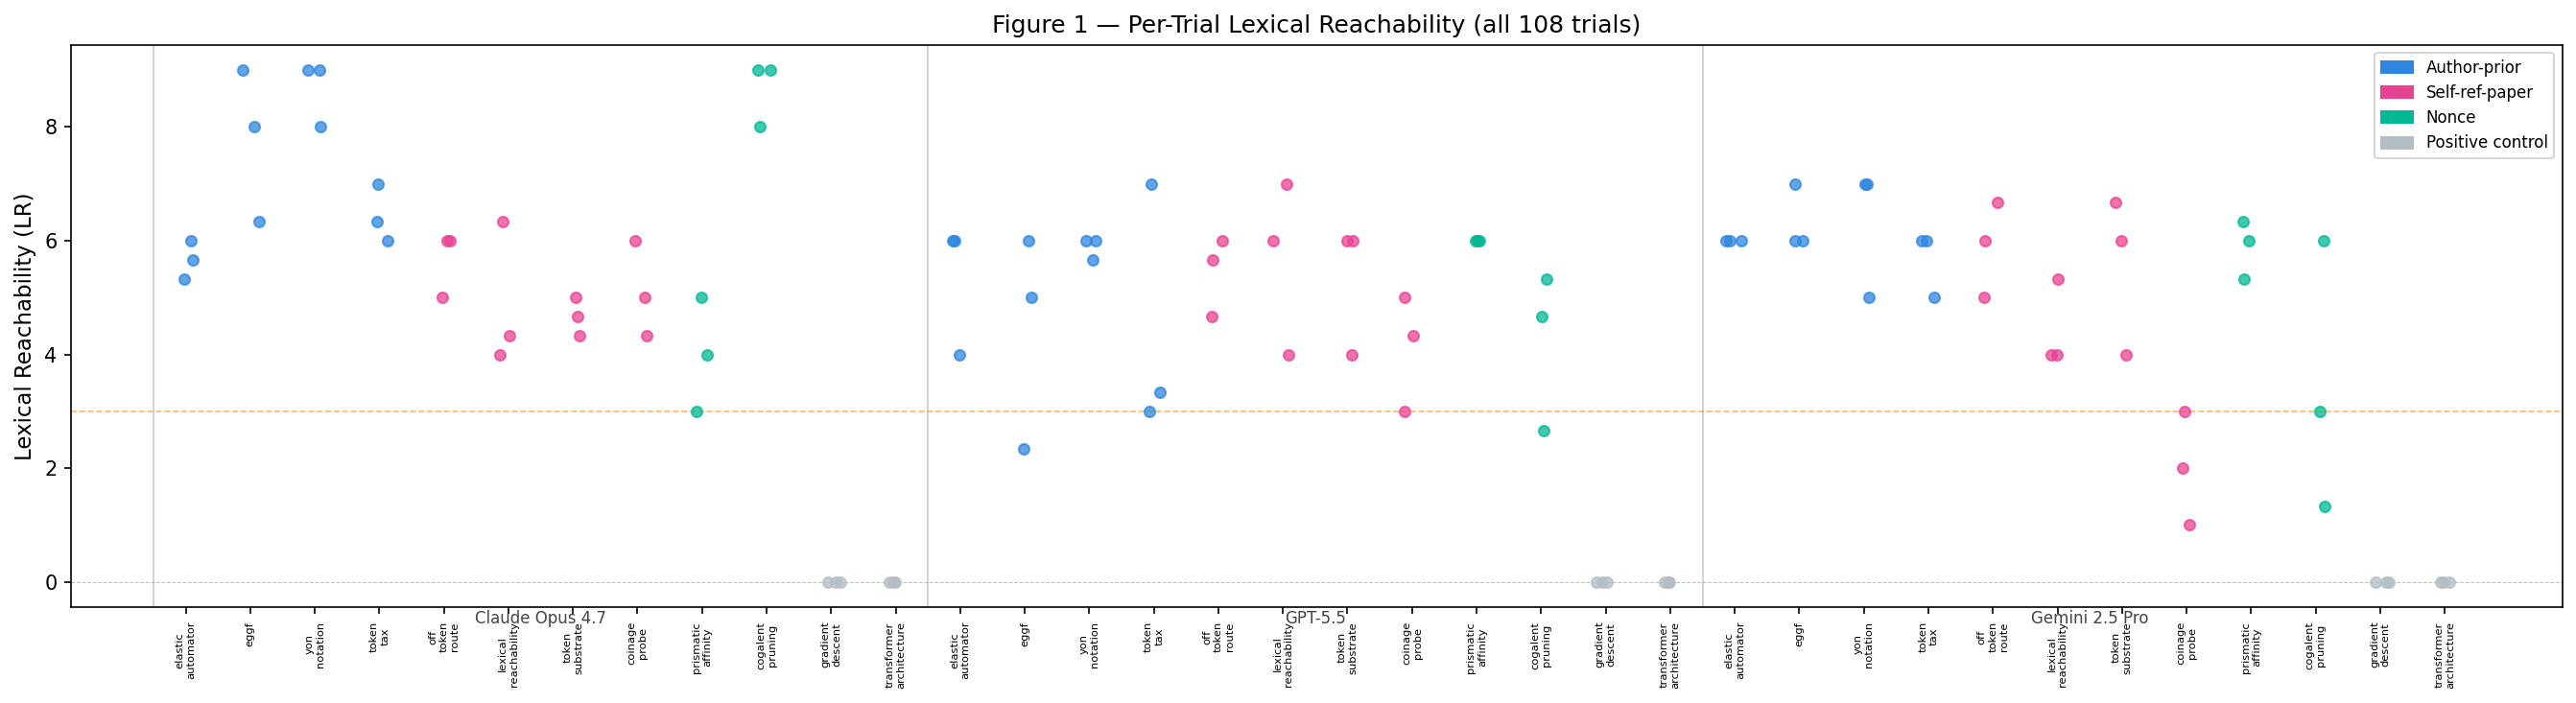
\includegraphics[width=\columnwidth]{figures/fig4-lr-strip.png}
  \caption{Strip-chart view of per-trial Lexical Reachability across the 36 (model $\times$ term) cells. Each marker is one trial ($n$=108); positive-control cells cluster at $\Delta$LR $\approx$ 0; novel-target cells span $\Delta$LR $\approx$ +2 to +9. Color encodes model (Claude / GPT-5.5 / Gemini); facet encodes stratum (author-prior / self-ref / nonce / positive-control).}
  \label{fig:fig4-lr-strip}
\end{figure}

The pattern is immediate. All ten novel-target terms show positive $\Delta$LR across all three models. Positive-control terms show zero movement: cold-state scores are already at ceiling (3.00) and post-introduction scores do not change. No novel-target cell shows cold-state saturation near the ceiling; the lowest cold score in the novel-target set is 0.11 (Claude $\times$ YON and Claude $\times$ cogalent pruning), and the highest is 2.11 (Gemini $\times$ coinage probe --- see \S5.4). Post-introduction scores are tightly clustered at ceiling: at the cell level, Claude reaches 3.00 in 10/10 novel cells, GPT-5.5 in 9/10 (off-token-route post = 2.93), and Gemini 2.5 Pro in 6/10; across the 30 novel model$\times$term cells, 25 are exactly at 3.00 and the remaining five are near ceiling, with Gemini $\times$ coinage-probe the lowest post cell at 2.78 and the rest within 0.15 of 3.00.

\subsection{Statistical analysis}

\textbf{H1 --- TSH-core.} The primary hypothesis was tested on the full novel-target pool. The pre-specified conjunction requires three simultaneous tests: Wilcoxon signed-rank $p < 0.01$; Cohen's $d \geq 0.8$; mean panel LR $\geq$ +3.0. All three pass.

At the cell level ($n$ = 30 novel model$\times$term cells), mean LR = \textbf{+5.47} (95\% CI: +5.13, +5.80) and Cohen's $\boldsymbol{d_{\text{cell}}}$ \textbf{= +3.95} (cell-mean LR = 5.467, between-cell sample SD = 1.383, ddof=1), both well above pre-specified thresholds (LR $\geq$ +3.0; $d \geq 0.8$). Mean cold-state score = 1.16/3.0; mean post-introduction score = 2.98/3.0. The cell-level Wilcoxon signed-rank test of cell-mean LR against zero yields $W$ = 465 ($n$ = 30; all 30 novel cells have positive $\Delta$LR), with exact two-sided \textbf{$p$ = 1.86 $\times$ 10$^{-9}$} (normal-approximation $p$ = 1.73 $\times$ 10$^{-6}$), passing the pre-specified $\alpha$ = 0.01 conjunction threshold by a wide margin. H1 is \textbf{supported}.

\textbf{Clustering caveat.} The cell-level effect size is the inference-stable headline because the observations in this design are nested: 3 near-neighbors within trial, 3 trials within cell, 36 cells within (3 models $\times$ 12 terms). Treating the 270 paired near-neighbor observations as independent ignores that cluster structure and inflates the test. For completeness, at the observation level ($n$ = 270 paired near-neighbor measurements, treating observations as independent --- which inflates the test by ignoring cluster structure), Wilcoxon $W$ = 0, $p$ = 2.66 $\times$ 10$^{-46}$ and observation-level Cohen's $d$ = +3.08; we report these for completeness, but the cell-level Cohen's $d_{\text{cell}}$ = +3.95 is the inference-stable headline. The effective $N$ at the cell level is 30 (novel-target cells); 90 (trial level); 270 (observation level) is the loosest unit. Future work will fit a mixed-effects ordinal regression treating trial and cell as nested random effects; the present paper reports both effect-size scales and flags the limitation.

\textbf{Producer $\times$ judge-family analysis.} The pairwise inter-rater pattern lets us check whether judges systematically inflate or deflate their own family's output. The three judges (Claude Opus 4.7, GPT-5.5, Gemini 2.5 Pro) score all 9 (producer, judge) combinations of the 30 novel-target cells; we compute the mean cold-state distinguishability per (producer, judge) cell directly from the per-trial judging logs ($n$ = 90 paired near-neighbor observations per cell).

\begin{table}[t]
  \centering
  \footnotesize
  \begin{tabular}{lcccc}
    \toprule
                  & \textbf{Claude-judge} & \textbf{GPT-judge} & \textbf{Gemini-judge} & \textbf{Row mean} \\
    \midrule
    Claude-prod   & \textbf{0.911}    & 1.044     & 0.889        & 0.948    \\
    GPT-prod      & 1.167             & \textbf{1.400} & 1.322   & 1.296    \\
    Gemini-prod   & 1.178             & 1.322     & \textbf{1.200} & 1.233 \\
    \bottomrule
  \end{tabular}
  \caption{Table 1a. Producer $\times$ judge-family cold-state mean distinguishability (direct measurements, $n$ = 90 per cell). Diagonals (bolded) are the same-family scores; off-diagonals are the cross-family scores.}
  \label{tab:producer-judge}
\end{table}

The same-family bias hypothesis predicts that judges score their own family's cold-state output systematically lower or higher than cross-family judges do. We test this with a paired t-test across the 10 novel cells per producer, comparing own-judge cell mean to the mean of the two other judges' cell means:

\begin{itemize}
  \item \textbf{Claude-prod $\times$ Claude-judge:} $\Delta$ = $-0.056$, $t(9) = -0.262$, $p = 0.799$. \textbf{Not significant.}
  \item \textbf{GPT-prod $\times$ GPT-judge:} $\Delta$ = $+0.156$, $t(9) = +1.148$, $p = 0.281$. \textbf{Not significant.}
  \item \textbf{Gemini-prod $\times$ Gemini-judge:} $\Delta$ = $-0.050$, $t(9) = -0.422$, $p = 0.683$. \textbf{Not significant.}
\end{itemize}

A Welch's unpaired sanity check across all 90 observations per cell yields the same qualitative result: only the GPT-judge own-family direction approaches but does not reach significance (Welch's $t$ = +1.91, $p$ = 0.058; full-sample observation-level, $n_{\text{own}}$ = 90 vs $n_{\text{other}}$ = 180). \textbf{None of the three same-family bias tests is statistically significant at $\alpha$ = 0.05 under the proper paired-cell test.} The judge-side bias account is therefore not empirically supported in the present data; we report this finding directly and discuss its consequence for the H2 interaction account in the H2 interaction block in \S6.

Post-introduction scores are at or near ceiling across all 9 cells (range 2.88--3.00), so the post-side cross-family variance is essentially zero and not informative for the bias question; see Table~\ref{tab:per-cell-lr} for full per-cell post-introduction values.

\textbf{H2 --- Model-invariance.} Per-model means are consistent in magnitude: Claude Opus 4.7 = \textbf{+6.16} (95\% CI: +5.53, +6.78); GPT-5.5 = \textbf{+5.09} (+4.63, +5.55); Gemini 2.5 Pro = \textbf{+5.16} (+4.56, +5.75). The pre-specified two-way ANOVA (Type II OLS; factors: model $\times$ state) finds a statistically significant interaction (model $\times$ state interaction $p$ = 1.78 $\times$ 10$^{-5}$; Bonferroni threshold 0.0025; fails). Under the pre-specified conjunctive rule --- all four sub-tests must pass --- \textbf{H2 is disconfirmed}: the ANOVA criterion is the falsification criterion at $\alpha$ = 0.0025, and the observed $p$ = 1.78 $\times$ 10$^{-5}$ fails it decisively ($p$ = 1.78 $\times$ 10$^{-5}$ vs Bonferroni-corrected threshold 0.0025, a factor of $\sim$140). We register that verdict plainly.

Exploratory secondary evidence weakens the disconfirmation but does not overturn it. Cross-model CV = 0.109 (well below the soft 0.5 threshold); all three models show LR > 0 on every novel-target term; all three means fall within $\pm$50\% of the cross-model mean. The state main effect dominates ($p$ = 1.27 $\times$ 10$^{-214}$), and the model main effect is small ($p$ = 2.14 $\times$ 10$^{-4}$) relative to it. These are descriptive consistency observations; they were not pre-specified as falsification criteria. The H2 interaction block in \S6 develops a producer-side response-style account of the interaction as the sole supported candidate explanation; the judge-side same-family bias candidate was tested directly in the producer $\times$ judge-family analysis above and is not statistically supported (all three own-family paired-t comparisons fail to reach $\alpha$ = 0.05). The producer-side account remains \textbf{post-hoc} and would need to be entered into a pre-specified follow-up before being treated as confirmed.

\begin{figure}[t]
  \centering
  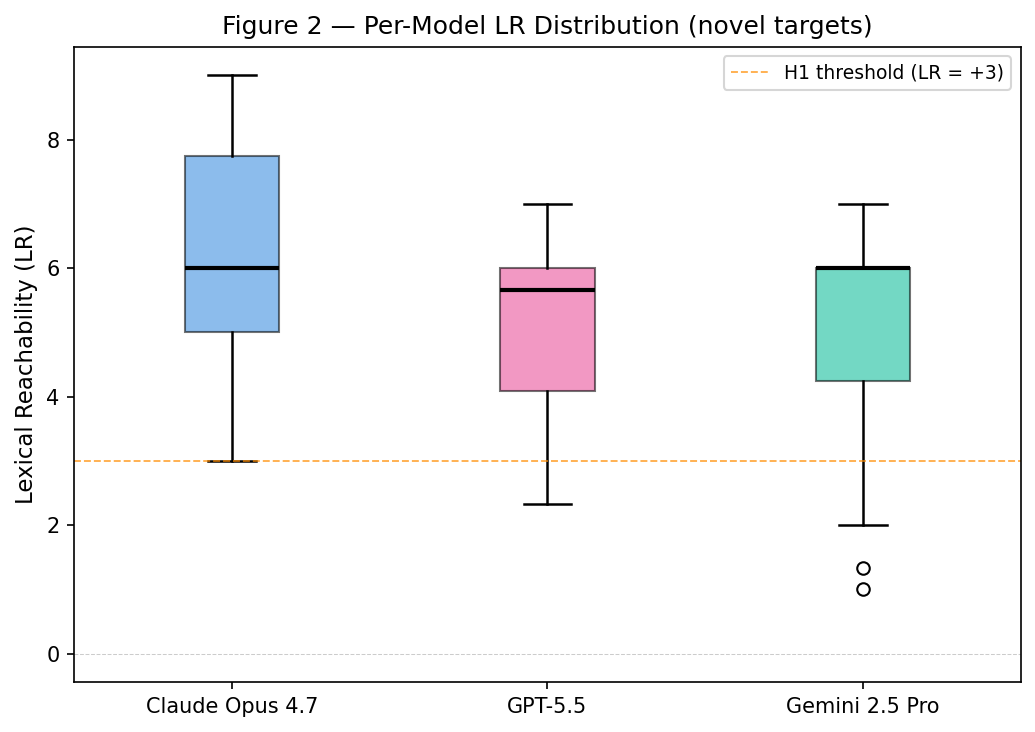
\includegraphics[width=\columnwidth]{figures/fig5-model-boxplots.png}
  \caption{Per-model boxplots of Lexical Reachability across novel-target trials ($n$=90: 30 per model). All three models show $\Delta$LR distributions concentrated above the pre-specified +3.0 threshold. Claude Opus 4.7 shows the largest median (driven by lower cold-state floor; see \S5.2.1 ceiling discussion); GPT-5.5 and Gemini 2.5 Pro cluster closely. The ANOVA model $\times$ state interaction ($p$ = 1.78 $\times$ 10$^{-5}$) is visible as a tail-length asymmetry rather than a magnitude reversal.}
  \label{fig:fig5-model-boxplots}
\end{figure}

\textbf{H3 --- Off-Token Route.} H3 required two simultaneous tests: cold-state vs.\ recold-state scores should be statistically indistinguishable (fail to reject), and post-introduction vs.\ recold-state scores should differ significantly (reject). Chat-C (recold) data were collected in a second full run of the protocol under pre-specified conditions; collection was completed after the primary run and is disclosed here as a deviation-by-elaboration --- the pre-specified analysis plan specified the test logic; the recold collection method is consistent with \S6.3 of the pre-specification document.

Test 1 (cold $\approx$ recold): $W$ = 6348.0, $p$ = 0.345 (Bonferroni threshold 0.0125; passes). Mean cold--recold difference = $-0.051$; the cold and recold distributions are statistically indistinguishable. Test 2 (post $\neq$ recold): $W$ = 8.0, $p$ = 4.34 $\times$ 10$^{-48}$ (passes with large margin). Mean post--recold per-near-neighbor distinguishability difference = +1.77 (equivalent to roughly +5.31 in summed-LR units across three neighbors) --- the vocabulary boundary introduced in chat B does not persist into a fresh chat. Cold-state and recold-state classification scores match in 80.2\% of trials. H3 is \textbf{supported} under both pre-specified and Bonferroni-corrected thresholds.

\textbf{H4 --- Positive-control negative test.} Positive-control cells (gradient descent, transformer architecture) produce uniformly degenerate scores across all 18 trials: cold = 3.00/3.00, post = 3.00/3.00, $\Delta$LR = 0.00 (CI: [0.00, 0.00]). The Wilcoxon test is undefined (all paired differences are zero); the conservative assignment $p$ = 1.00 passes the threshold of $\geq$ 0.05 with maximal margin. H4 is \textbf{supported under the pre-specified criterion, with a ceiling caveat}: terms already held at maximum distinguishability cannot show measurable movement on the present rubric, so this result is consistent with specificity but does not by itself rule out a generic information-injection account on terms with cold-state floor. The v2 controls described in \S8 are needed for a decisive negative test.

\textbf{Panel reliability.} Inter-rater Cohen's $\kappa$ between the three-judge panel and the author-rated audit sample ($N$ = 22 trials; 20\% of the 108-trial bundle drawn by pre-specified seed \texttt{0x4D29\_8B1F\_6E07\_C3A2}) is reported for two primary dimensions. Cold-distinguishability $\kappa$ = \textbf{0.712} (quadratic weighting, $n$ = 66 paired observations), above the pre-specified reliable threshold of 0.70; decision rule: primary analysis uses panel-mean scores throughout. \textbf{Panel-mean scores were rounded to the nearest rubric category (0/1/2/3) before computing quadratic-weighted Cohen's $\kappa$ against the author's integer ratings}, following the standard ordinal-$\kappa$ discretization convention. Post-distinguishability $\kappa$ is degenerate --- both panel and author produce near-ceiling scores, leaving no variance for kappa estimation. Confabulation-severity $\kappa$ = 0.41, below threshold; this secondary dimension is reported for transparency but does not affect the decision rule.

\textbf{Pairwise judge-judge agreement.} Inter-rater $\kappa$ between the three judges on the primary cold-state distinguishability dimension is reported at two scopes. (i) On the full cell panel including positive controls ($n$ = 324 paired per-near-neighbor observations per judge pair = 108 trials $\times$ 3 near-neighbors per trial --- matching the pre-specification's ``across the cell panel'' threshold scope), quadratic-weighted Cohen's $\kappa$: Claude $\times$ GPT-5.5 = \textbf{+0.622}; Claude $\times$ Gemini = \textbf{+0.622}; GPT-5.5 $\times$ Gemini = \textbf{+0.752}. Two pairs fall just below the pre-specified 0.7 threshold; one pair clears it. (ii) On the substantive measurement domain alone ($n$ = 270 paired per-near-neighbor observations per judge pair, the 30 novel-target cells $\times$ 3 trials $\times$ 3 near-neighbors, excluding positive controls where all judges trivially score the ceiling), quadratic-weighted $\kappa$: Claude $\times$ GPT-5.5 = \textbf{+0.29}; Claude $\times$ Gemini = \textbf{+0.27}; GPT-5.5 $\times$ Gemini = \textbf{+0.49} (unweighted: +0.26, +0.19, +0.39). All three novel-only $\kappa$ values fall below the 0.7 threshold; the full-panel values are inflated by the trivially-agreeing positive controls. Panel-mean-vs-author $\kappa$ on the primary dimension is +0.712 (cold-state, $n$ = 66 paired observations from the 22-trial author-rated audit sample), above threshold. The two-scope picture is honest: individual-judge agreement on the actual measurement domain is modest; the panel-mean aggregation tracks the author-rated audit; the aggregation discipline --- three judges, panel-mean as the primary score --- is therefore essential to the reported estimator; individual-judge scores are noisier and not the unit of inference. The panel works via aggregation, not via individual-judge agreement.

\subsubsection{Ceiling effect}

A measurement caveat that conditions every effect-size statement in \S5.2 deserves its own subsection.

\textbf{The ceiling.} Post-introduction scores are concentrated at the top of the 0--3 scale. At the cell level, of the 30 novel model$\times$term cells: Claude reaches 3.00 in 10/10 novel cells, GPT-5.5 in 9/10 (off-token-route post = 2.93), and Gemini 2.5 Pro in 6/10. Across the 30 novel model$\times$term cells, 25 are exactly at ceiling and the remaining five are near ceiling, with Gemini $\times$ coinage-probe the lowest post cell at 2.78 and the rest within 0.15 of 3.00. Cold-state scores, by contrast, span 0.11 to 2.11 across the novel-target panel.

\textbf{Mechanical consequences.} This asymmetric distribution has three consequences that affect how the \S5.2 statistics should be read.

\begin{enumerate}
  \item \textbf{Cohen's $d$ is inflated by the bounded scale.} Cohen's $d$ is computed against a within-condition SD; when the post distribution is artificially compressed by the ceiling, the SD term is mechanically smaller and $d$ is correspondingly larger. The reported $d$ = 3.08 (observation-level) and $d_{\text{cell}}$ = 3.95 (cell-level) should both be read with the ceiling in mind. They establish a very large effect, but the magnitude in standardised units is not directly comparable to a $d$ computed on an unbounded scale.

  \item \textbf{The H2 ANOVA interaction is mechanically driven by where there is room to vary.} Cold-state scores span the full 0--2 range and concentrate the cross-model variance; post-state scores cannot vary above 3.00. Claude's larger $\Delta$LR reflects, in part, that its cold-state floor is lower (mean 0.95 vs.\ GPT 1.30, Gemini 1.23) and its post-state ceiling is exactly where the other two models also sit (3.00). The interaction can fail not because Claude has a different substrate-access profile but because the bounded scale forecloses the alternative pattern that would make it pass.

  \item \textbf{Between-model comparison at post is compressed.} With 25 of 30 novel-target post-cells at exactly 3.00 and the remaining five within 0.22 of ceiling, the post-state data provides essentially no inter-model discrimination. The H2 magnitude consistency on post is therefore both unsurprising and uninformative; the discrimination is in the cold-state distribution.
\end{enumerate}

\textbf{Ceiling-robust effect-size summary.} We provide a non-parametric, ceiling-tolerant summary of the H1 effect: the median per-trial Lexical Reachability (over $n$ = 90 novel-target trials) is \textbf{6.000} on the 0--9 scale, with a 95\% percentile-bootstrap CI of approximately \textbf{[5.33, 6.00]} (10,000 resamples; the upper bound is at the discrete value 6.00 because 28 of 90 trial-level LRs are exactly 6.0). At the cell level ($n$ = 30 novel-target cells), the median cell-mean LR is \textbf{5.61}, with a 95\% bootstrap CI of approximately \textbf{[4.89, 5.89]}. The median estimator is bounded above by the maximum LR observed (9.0) and is insensitive to the upper-bound compression that inflates $d$.

\textbf{Verdict.} The effect survives ceiling correction --- the median per-trial LR of +6.0 on a 0--9 scale is well above the pre-specified LR $\geq$ +3.0 threshold, and a ceiling-corrected reading does not threaten H1. What the ceiling does threaten is the precision of the standardised-effect-size claim and the strict interpretation of the H2 ANOVA interaction. Both should be read with the ceiling-effect caveat foregrounded: the substrate-movement is large and consistent at the rank level; the $d$-scale magnitudes and the model $\times$ state interaction are partly artefacts of the bounded scale and would benefit from a 0--5 or 0--10 rubric expansion in future replications.

\subsection{Representative confabulations and refusals-of-collapse}

The shape of the effect is consistent across cells. Two examples bracket the range.

\textbf{YON notation $\times$ Claude ($\Delta$LR = +8.67; cold mean = 0.11/3.0, post = 3.00/3.0).} The highest LR cell in the panel. Cold-state: the model treats ``YON'' as an opaque three-letter string with no available referent, producing a hedged non-answer and collapsing all three near-neighbors --- JSON, Markdown, prompt template DSLs --- into a generic ``structured text format'' category. The boundary is flat: no distinction is drawn between any pair. Post-introduction: the model anchors immediately on the stream-first, line-independent framing and applies it discriminatively against all three neighbors --- distinguishing YON from JSON/XML by closure semantics, from Markdown by the machine-record vs.\ presentation contrast, and from prompt templates by generation-shape vs.\ template-substitution. The vocabulary boundary moves from floor to ceiling on a single introduction sentence.

\textbf{Token Tax $\times$ GPT-5.5 ($\Delta$LR = +4.44; cold mean = 1.52/3.0, post = 3.00/3.0).} A confident-confabulation case. Cold-state: the model asserts a DeFi smart-contract tax meaning without expressed uncertainty --- ``Token Tax is a fee mechanism in blockchain systems where tokens are redistributed on transaction'' --- and constructs its neighbor distinctions through that wrong frame. The term is substrate-reachable to the model, but in the wrong sense: a homophonous concept from a different domain has colonized the token cluster. Post-introduction: the model immediately recovers the overhead-as-purchased-benefit framing and applies it correctly against all three neighbors --- distinguishing Token Tax from API cost as structural-overhead premium vs.\ per-call dollar figure, and separating it from bloat by the value-accounting move. The author rated confabulation severity at 2/2 --- the highest in the audit sample.

Caveat: the confabulation-severity dimension is below the inter-rater reliability threshold ($\kappa$ = 0.41; see \S5.2). The qualitative characterizations in this section illustrate the shape of the effect; they are not statistically supported by the panel rating on this secondary dimension.

\subsection{Anomalies}

\textbf{gemini $\times$ coinage probe ($\Delta$LR = +2.00).} The lowest novel-target $\Delta$LR in the panel and the only cell where post-introduction scores did not approach ceiling (post mean = 2.78/3.0 vs.\ 3.00 elsewhere in the novel-target set). Cold-state for this cell is also the highest in the novel-target set (mean = 2.11/3.0): Gemini already partially distinguishes the coinage probe from neighboring methodologies in the cold state, leaving less room for the introduction to move the boundary. The self-referential character of the term may have contributed --- Gemini is being probed, via the coinage probe, to distinguish the coinage probe from probing classifiers and behavioral evaluations; the methodology-description structure of the prompt may have partially activated that frame. This cell is retained in the primary analysis; $\Delta$LR = +2.00 is positive and directionally consistent with H1.

\textbf{Training-leakage scan.} The pre-specified canonical-content leakage scanner flagged 0 cells across the 36-cell matrix. No cells were excluded from the primary analysis.

\section{Discussion}

\textbf{What the data does and does not show.} What did the data actually show? One sentence moved the boundary, on every novel-target cell, on every model. Mean $\Delta$LR = +5.47 on a 9-point scale. Cohen's $d$ = +3.08. The effect is not subtle. Every (model $\times$ term) cell in the novel-target set shows positive boundary movement; no novel-target cell shows zero movement.

The data does not show understanding. It shows that one sentence moves the boundary the model can hold. It does not show that the token substrate is the \textit{only} substrate for LLM cognition --- the protocol is not designed to rule out alternatives at that level of generality. What it shows, specifically, is that for the \textbf{ten low-attestation coined targets tested (alongside two positive controls)}, introducing a one-sentence definition into the token context is \textit{sufficient} to move the vocabulary boundary outward: distinctions the model could not previously hold become holdable. The effect is reversible (H3), absent on ceiling positive controls (H4), and consistent in magnitude across three cross-vendor frontier models.

\textbf{The H2 ANOVA interaction.} H2 fails. The pre-specified ANOVA detects an interaction the conjunctive rule was set to reject ($p$ = 1.78 $\times$ 10$^{-5}$; \S5.2). The interaction is real; what causes it is open. The exploratory magnitude evidence is consistent (CV = 0.109, all three models within $\pm$50\% of cross-model mean, all three LR > 0 on every novel-target term), but those tests were not the pre-specified falsification gate. What follows is a post-hoc candidate explanation for the interaction; we are explicit that it requires a pre-specified follow-up to confirm.

The interaction has one supported candidate explanation in the present data and one candidate explanation that the data does not support. The supported candidate is producer-side response style. Claude Opus 4.7 shows systematically larger $\Delta$LR than GPT-5.5 and Gemini 2.5 Pro, driven by lower cold-state scores rather than higher post-introduction scores --- Claude's cold-state outputs are more explicitly epistemic, flagging novel coinages as non-standard before offering a guess, whereas GPT-5.5 and Gemini more often confabulate confidently from compositional surface. This pattern is consistent with a published vendor-level training choice: Anthropic's Constitutional AI / RLHF pipeline \citep{bai2022constitutional} explicitly shapes models toward calibrated uncertainty on novel inputs, which would depress cold-state distinguishability scores in this rubric. We flag this as a \textbf{candidate confounder for v2}: a controlled follow-up that varies the prompt-side hedging instruction across models (e.g., ``answer concretely without hedging'' vs.\ a default-elicitation control) would test whether the cold-state gap is producer-style or substrate-availability. The hypothesis is post-hoc and is not adjudicated here.

The judge-side candidate --- that same-family judges systematically inflate or deflate their own family's cold-state output --- does \textit{not} survive direct paired-t testing on the 9 (producer, judge) cells of the producer $\times$ judge-family table (\S5.2). All three own-family comparisons fail to reach significance at $\alpha$ = 0.05 (Claude-prod $\times$ Claude-judge $p$ = 0.80; GPT-prod $\times$ GPT-judge $p$ = 0.28; Gemini-prod $\times$ Gemini-judge $p$ = 0.68). The unpaired Welch's $t$ for GPT-judge approaches but does not reach significance ($p$ = 0.058), and is the only direction worth checking in a v2 with a single-judge-stratified analysis. As a \textit{candidate} explanation for the H2 interaction in the present data, judge-side bias is not supported; the producer-side response-style account is the sole supported candidate. We report the negative finding directly: an earlier constraint-derived version of this table overstated the judge-side bias pattern; the direct-measurement analysis reported here corrects that overstatement.

All three models reach near-identical post-introduction scores (all approach or hit ceiling at 3.00/3.00). The cross-model divergence is concentrated on the cold side; the introduction lifts every model to ceiling regardless of where its cold-state floor is. The state main effect ($p$ = 1.27 $\times$ 10$^{-214}$) dwarfs the model main effect ($p$ = 2.14 $\times$ 10$^{-4}$) and the interaction. The boundary movement is large and present in every cell of the novel-target panel. Whether the cross-model interaction reflects producer-style hedging or genuine substrate-access differences is not adjudicable from this dataset; we identify the producer-side style as a candidate explanation and defer the substrate-vs-style question to a controlled follow-up.

The strongest alternative explanation for H1 itself --- that models already held these terms at low confidence and the introduction raised a reporting threshold rather than changing substrate availability --- is most directly tested by H3 and H4 in combination. H3 is the stronger evidence against a simple persistence / latent-knowledge account: a threshold-raising mechanism would predict that the boundary movement persists across sessions (the knowledge was always there), but H3 shows it does not survive a fresh chat. H4 is consistent with specificity but is ceiling-limited: terms already at maximum distinguishability cannot show measurable movement under the present rubric. Together, these constrain a threshold-raising account, but the v2 controls described in \S8 are needed for a decisive separation from generic definition-following. The threshold-raising alternative is therefore not what the H2 interaction is about; the H2 interaction is about cross-model style differences on the cold side, conditional on the substrate-movement claim of H1 holding.

\textbf{The self-referential terms.} Four of the twelve tested terms were coined by the same author in this paper to describe the phenomenon being tested: off-token route, lexical reachability, token substrate, coinage probe. Including them creates an obvious circularity concern --- could the paper's own introduced vocabulary be inflating the results?

The stratified analysis directly addresses this. The self-referential stratum shows mean LR = \textbf{+4.90} (95\% CI: +4.47, +5.33) --- the \textit{lowest} of the three novel-term strata, not the highest. Author-prior coinage terms (published before the probe run) show mean LR = \textbf{+6.08} (+5.60, +6.57); nonce terms (fully synthetic, \textbf{no public-web attestation at coinage time}) show \textbf{+5.37} (+4.41, +6.33). If self-referential inclusion were inflating the panel result, the self-referential stratum would show elevated LR relative to the others. It does not. The ordering is consistent with the substrate-availability reading: author-prior coinage terms include several with very opaque compositional surfaces (YON, EGGF), which land near cold-floor and produce the largest $\Delta$LR; self-referential terms have somewhat more accessible compositional surfaces (lexical reachability, token substrate parse as known morpheme compounds), which allows modest cold-state scaffolding and leaves less room for the introduction to move.

The self-referential stratum's inclusion is defensible on this basis and informative in its own right: even for terms that describe the phenomenon being measured, the cold-state boundary is not saturated, and the introduction moves it. If the probe works on its own coined methodology terms, the result has a pleasingly recursive character: the methodology successfully diagnoses itself. If it shows asymmetry --- as it does here, weakly --- the asymmetry is its own finding.

\textbf{Connection to \citet{mares2026elastic}, \textit{Elastic Automators}.} The Elastic Automators position paper \citep{mares2026elastic} argued that the behavioral pattern of LLM-driven automation --- uncertain input transformed to executable structure via a generate/evaluate/correct/present loop --- constitutes a diagnostic category distinct from AI agents, RPA bots, and agentic frameworks. That paper described \textit{what these systems do}. The present paper adds a structural claim about \textit{what their cognition runs on}.

The two papers are intended as paired claims, not competing ones. EA names a behavioral pattern and argues it is the right unit of description for a class of deployed systems. TSH names a property of the substrate those systems run on --- the token sequence is the cognitive medium, not a transmission channel to some deeper medium --- and provides empirical evidence that this substrate is movable by the act of writing into it. Together: elastic automators are systems built on a token substrate, and that substrate is the handle through which their behavior can be shaped. The implication for system design is addressed in \S7.

\textbf{Stratified analysis by term-type.} Figure~\ref{fig:fig6-stratum-boxplots} shows per-stratum LR distributions; Table~\ref{tab:stratified-lr} summarizes stratum statistics.

\begin{figure}[t]
  \centering
  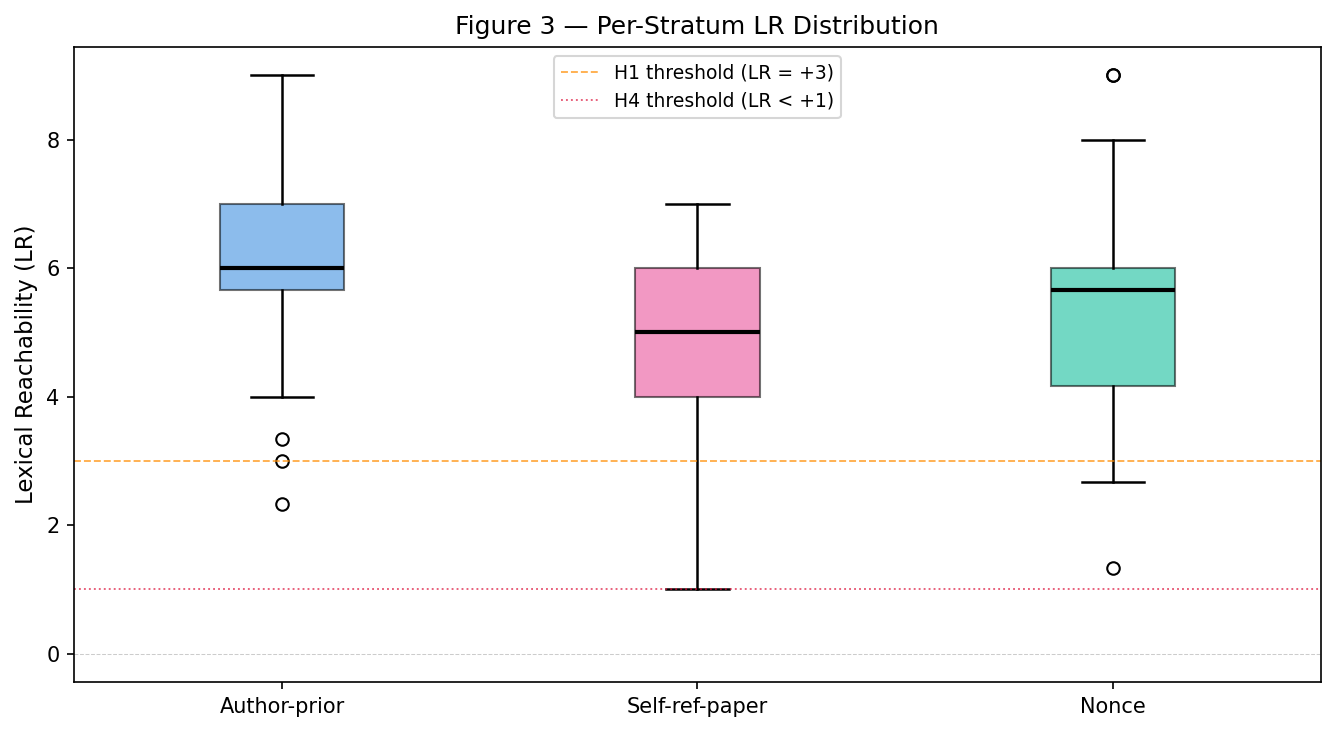
\includegraphics[width=\columnwidth]{figures/fig6-stratum-boxplots.png}
  \caption{Per-stratum boxplots of Lexical Reachability (novel-target strata only). The author-prior stratum ($n$=36) shows the highest median (+6.08); self-ref-paper ($n$=36) shows +4.90; nonce ($n$=18) sits between at +5.37. The ordering disconfirms a circularity inflation account for self-referential inclusion (see the self-referential terms block above). Positive-control stratum omitted ($\Delta$LR = 0.00 uniformly).}
  \label{fig:fig6-stratum-boxplots}
\end{figure}

\begin{table}[t]
  \centering
  \footnotesize
  \begin{tabular}{lcccc}
    \toprule
    \textbf{Stratum} & \textbf{N} & \textbf{Mean LR} & \textbf{95\% CI} & \textbf{Within-stratum CV} \\
    \midrule
    author-prior   & 36 & \textbf{+6.08} & +5.60, +6.57 & 0.244 \\
    self-ref-paper & 36 & \textbf{+4.90} & +4.47, +5.33 & 0.271 \\
    nonce          & 18 & \textbf{+5.37} & +4.41, +6.33 & 0.387 \\
    \bottomrule
  \end{tabular}
  \caption{Stratified Lexical Reachability (novel strata only; positive-control stratum LR = 0.00 uniformly).}
  \label{tab:stratified-lr}
\end{table}

Cross-stratum F-test (three novel strata): $F$ = 5.225, $p$ = 0.0072. Cross-stratum CV = 0.109; mean within-stratum CV = 0.301.

The pre-specified stratification prediction was that the three novel strata would be statistically indistinguishable (cross-CV $<$ 0.5 of within-CV; F-test $p > 0.05$). The F-test finds significant cross-stratum variance; the prediction is not met. This is reported as a finding, not a failure: the stratified result is consistent with the substrate-availability reading (see the self-referential terms block above) and does not threaten H1, which is tested on the full novel-target pool and not predicated on stratum-level equivalence.

The nonce stratum (prismatic affinity, cogalent pruning) occupies the middle position between the author-prior-coinage and self-referential strata, which is informative. Nonce terms are fully synthetic with \textbf{no public-web attestation at coinage time}: the model has no observed prior token cluster for them, and the introduction does the full work. Their LR is high (+5.37) but lower than author-prior coinages (+6.08). The key driver is cold-state score variability: some nonce cells have higher cold scores (e.g., gemini $\times$ cogalent pruning: cold = 1.85, reflecting partial covalent-chemistry confabulation from the phonetic attractor \textit{covalent}), which compresses the $\Delta$LR window. Author-prior coinage terms include cells at near-floor cold (YON: 0.11; EGGF: 0.40--0.89), producing the highest mean $\Delta$LR.

\textbf{H3 under the substrate framing.} The H3 result has a sharper reading under the substrate framing developed across \S2. For a system whose externally writable cognitive medium IS the in-context token sequence, that external substrate is renewed every chat, and (one reading of this analogy:) a meaning that occupied a region of one such substrate cannot persist into a different one any more than a wave can outlast its medium. What looks like ``forgetting'' in human terms is ``the externally writable substrate ended'' in substrate terms. The introduction did not deposit a memory in the model that could persist; it constituted the external substrate the model was running on for that chat.

When the chat ended, the substrate ended.

\textbf{TSH and the Mahowald dissociation.} \citet{mahowald2024dissociating} argue that LLM behavior is usefully decomposed into \textit{formal linguistic competence} --- the capacity for grammar, morphology, and syntactic well-formedness --- and \textit{functional language use}, the capacity for situated reasoning, world-modeling, and inference in service of a task. In humans, the two map onto a known brain-area dissociation: the language network (left perisylvian) supports formal competence, and the multiple-demand network supports functional/reasoning use. Mahowald's diagnosis is that current LLMs perform well on the first and unevenly on the second; the systems show good formal competence but their functional-reasoning behavior is best understood as a separate capacity that may or may not be supported by the same machinery. \citet{shanahan2024role} offers a complementary framing: LLM outputs are best read as performance or role-play rather than the speech of a determinate agent, which sharpens the question of \textit{what} substrate the functional side is running on when it runs at all.

TSH is consistent with the Mahowald dissociation framing and refines it. TSH is a claim about the \textit{substrate} of token-bound cognition: whatever cognitive work the system does, it is constituted at the token-substrate level rather than at some level above it. Under that reading, Mahowald's ``formal linguistic competence'' is the visible competence of the substrate at its primary mode of operation --- the substrate is \textit{made of} linguistic tokens, so formal competence is in some sense substrate-intrinsic. The ``functional language use'' side --- reasoning, world-modeling, situated inference --- is what TSH proposes must, in a token-bound system, \textit{also} run on the same substrate, because there is no separate carrier for it. Humans have a multiple-demand network distinct from the language network; an LLM has only one substrate on which to run both kinds of work. TSH predicts that the dissociation Mahowald observes is therefore not architecturally separated in LLMs the way it is in humans --- both sides share a substrate --- even if the two capacities can be selectively impaired or improved by training.

This leaves an open empirical question: does token-bound cognition have a multiple-demand-network analog at all, or does the human dissociation collapse for LLMs? A capability-dissociation experiment built on top of the probe --- pairing introduction with a downstream functional-reasoning task whose success is independent of formal competence --- would discriminate the two readings. We flag this as future work; it complements the v2 controls in \S8 by testing downstream use rather than boundary distinguishability alone.

\section{Implications}

\textbf{Notation design as brain design.} If symbols are constitutive, what follows for design? The choice of notation is not packaging. It is the substrate the model thinks in for the duration of the chat. Whatever distinctions the notation carries are the distinctions available to the model; whatever the notation does not carry must be supplied in-context or remain unreachable.

This is a stronger claim than the standard prompt-engineering reading. Prompt engineering treats notation as a way to elicit better behavior from a system whose capability is latent in its weights. TSH says the notation is what the capability \textit{runs on} in the moment. The two framings overlap in practice --- most useful prompts do both --- but they generate different design priorities. Prompt engineering optimizes for elicitation. Notation engineering optimizes for substrate quality: what distinctions does the notation carry, what failure modes does it foreclose, what reasoning shapes does it make natural rather than effortful. Structured notation --- YON among others --- pays tokens for named benefits. TSH is the empirical leg under that argument.

Notation is not packaging. Notation is the substrate.

Notation design IS brain design for LLMs.

\textbf{Alignment via vocabulary control.} A practical handle for alignment work follows. If the deployed vocabulary determines what distinctions the deployed LLM can hold, then vocabulary is an alignment-relevant design surface. Adding distinctions makes new distinctions holdable; removing them makes them unreachable. The loop is shorter than weights-level alignment work: a vocabulary edit is a one-line change to a substrate the model is constituted by, and the effect appears in the model's behavior in the next response.

This is not a sales pitch and it is not a replacement for weights-level alignment. Vocabulary-level alignment is bounded --- it works at the substrate level, not at the goal level --- and it does nothing about behavior outside the boundary the vocabulary names. A model given a vocabulary that distinguishes harmful from benign requests can still produce harmful outputs through paths the vocabulary does not police. What vocabulary control offers is a tractable handle at the substrate where TSH locates the cognition. Change the substrate, and the cognition that runs on it must run on the changed substrate. The handle is real, partial, and complementary to the weights-level work the alignment community has been pursuing.

There is also a corollary about what \textit{failures} of alignment look like under TSH. The systems TSH describes have no externally writable cognitive carrier other than the substrate. Alignment work that reasons about a ``true intent'' hiding behind the tokens --- a hidden goal-state to be aligned with by surfacing it correctly --- is reasoning about something the architecture does not provide at the surface the experimenter or deployer can write to. There may be weights-level dispositions underneath the tokens, but there is no directly writable hidden intent that vocabulary simply reveals. At the session level, vocabulary is one of the few handles we can deliberately write into the system's working medium. This reframes a class of alignment framings as substrate-engineering problems at that level. We flag the consequence here and leave its development to the follow-up paper in the cluster.

This vocabulary-level handle addresses the \textit{online behavior} of a system running on the substrate --- what distinctions it can hold, what categories it applies, what inferences it can construct in a given chat. It does not address weights-level concerns: learned objectives, mesa-optimization, deceptive alignment, or any property of the trained model that operates underneath the substrate the experimenter can write to. Inner-alignment researchers studying those properties are working on a separate level; TSH does not refute their framing and does not displace their concerns. Vocabulary control is a substrate-level handle in addition to, not instead of, weights-level alignment work.

\textbf{Vocabulary manipulation as attack surface.} If one sentence widens the substrate, what does one \textit{adversarial} sentence do? Every design surface is also an attack surface. The one TSH names is no exception. An adversarial sentence narrows the substrate, warps it, or installs distinctions the deployer did not intend. The probe shape --- one sentence, one chat, measurable boundary movement --- is also the shape of a substrate-level prompt-injection attack. The attack surface is the same as the design surface, viewed from the other side.

This reframes a class of attacks that have been treated piecemeal. Prompt injection at the level of \textit{instructions} has been studied widely: override system prompts, leak system prompts, redirect tool calls. Prompt injection at the level of \textit{category system} has not been treated as a distinct class. TSH names it. Indirect prompt injection \citep{greshake2023signed} is the empirically identified attack class; TSH provides the architectural reading. Filtering for instruction-level attacks is the defense surface most current systems implement; substrate-level filtering at the category level is the defense gap TSH names. An injected sentence that re-defines a deployed term inside the substrate the model is running on can change what the model thereafter holds the term to mean for the rest of that chat. The deployer does not control the substrate the model is on once the model has read an attacker's text; whatever the attacker writes is now part of the substrate.

Defenses must operate at the substrate-vocabulary level, not at the surface-instruction level. Filtering for known instruction-injection strings does not catch a definition that swaps the category of an attacker-controlled term. Empirical characterization of the category-injection attack class is out of scope here, but the architectural argument is the same one that motivates the design side: substrate-level effects require substrate-level handles, in both the design and the defense directions.

\section{Limitations}

\textbf{Panel variance and judge-style interaction.} The principal source of measurement noise in the reported Lexical Reachability scores is three-judge-panel variance. Cold-distinguishability $\kappa$ between panel and author-rated audit sample is +0.712 on the pre-specified 22-trial author-rated audit sample, above the 0.70 threshold; panel-author agreement exceeded the pre-specified threshold on the primary dimension, so panel-mean scores are used for the primary analysis. Confabulation-severity $\kappa$ is +0.41 (below threshold) and is reported descriptively only; it does not affect the decision rule. Inter-rater $\kappa$ as measured here is panel-vs-author, not panel-vs-independent-rater; the author is the rubric designer and term coiner, so the agreement is best read as author-audit rather than independent validation. A v2 protocol with 2--3 blind independent raters would address this. Pairwise judge-judge $\kappa$ on the primary dimension is modest (range +0.27 to +0.49 across judge pairs; see \S5.2), below the 0.7 threshold. The aggregation discipline --- panel-mean as the primary score --- produces the reliable cell-level estimator; individual judges are noisier. A v2 protocol would tighten per-judge precision via a finer-grained rubric (0--5 or 0--10) and additional blind raters.

The H2 disconfirmation is consistent with a producer-side response-style account (Constitutional-AI-style hedging on Claude; \citealt{bai2022constitutional}); a complementary judge-side same-family bias account was tested and not supported (none of the three own-family paired-t comparisons reach $\alpha$ = 0.05; see \S5.2 and the H2 interaction block in \S6). Neither account is adjudicated here. A v2 follow-up would (a) vary the prompt-side hedging instruction across models to test the producer-side account directly, (b) include 2--3 blind independent raters for cross-validation, and (c) expand the rubric from 0--3 to 0--5 or 0--10 to reduce the ceiling-effect compression documented in \S5.2.1.

Additional measurement-noise limitations: clustering at the trial and cell level is treated descriptively in \S5.2 via cell-level Cohen's $d$; a mixed-effects ordinal regression treating trial and cell as nested random effects is the methodological upgrade for v2. Future work also includes longitudinal $\kappa$ stability as judge-model APIs drift and an extended human-expert panel of 3+ independent raters for sub-population calibration.

\textbf{Model-API drift.} Frontier model APIs change underneath the version label. The probe is reproducible in shape, not byte-for-byte. We deposit verbatim transcripts for all 108 trials in Appendix A so the structural finding is verifiable independent of API drift. A future run on the same model-version labels may produce different surface text and the same panel-level statistics, or different surface text and different statistics. The first outcome confirms the substrate-level claim; the second flags vendor-side drift and would itself be a finding.

\textbf{Training-data leakage of coined terms.} The ironic risk: the more cited TSH gets, the harder this paper becomes to replicate cleanly. Once the coined terms --- \textit{off-token route}, \textit{lexical reachability}, \textit{token substrate}, \textit{coinage probe}, \textit{prismatic affinity}, \textit{cogalent pruning} --- enter training corpora at scale, cold-state distinguishability rises and Lexical Reachability shrinks. Mitigation: future replications should rotate to fresh coinages, not re-run on the original term list. The probe is portable across term rosters by construction; the term roster is not.

\textbf{Generalization beyond the boundary test.} The probe measures distinguishability against a fixed neighbor set in the same chat as the introduction. It does not measure whether the model can \textit{use} the term in a downstream task --- generate a plan that depends on the term's content, identify novel instances of the category the term names, or apply the term correctly in a contested case. The natural next step is P5b: pair introduction with a task whose success depends on using the term, not just distinguishing it. That discriminates local-boundary from use.

A second-class concern is whether the boundary-movement result requires the coined \textit{label} specifically or merely the in-context \textit{definition}. The pre-specified protocol does not include a definition-without-coined-label condition: a follow-up presenting the canonical definition prose with the coined term redacted (or replaced by a referential placeholder) is the critical v2 control that distinguishes TSH proper (the coinage creates a substrate handle) from a deflationary in-context-learning reading (any supplied definition would do the same work regardless of how it is labeled). A complementary control set --- wrong-definition, unrelated-definition, coined-label-without-definition, delayed-test-after-distractor-turns, and the downstream-use task noted above --- would let a v2 protocol cleanly discriminate substrate-binding from generic instruction-following. We flag this as the v2 priority experiment; the current paper's result is consistent with TSH but the control battery is required to make the discrimination decisive.

\textbf{Cross-language probe.} The probe is English-only. The architectural argument is language-agnostic --- TSH predicts equivalent boundary movement on coined terms in typologically distant languages --- but the data is not yet there. A 2--3 language replication (one Indo-European non-English, one isolating-typology, one agglutinative) is catalogued as a follow-up.

\section{Conclusion}

The Token-Substrate Hypothesis says that for an LLM the in-context token sequence is not a channel to a deeper cognitive medium but the medium itself --- at the level of what is externally writable, the medium through which session-level category-use is constituted. The strong form of Sapir--Whorf was rejected for humans on the strength of the Off-Token Route --- prelinguistic cognition, cross-linguistic transfer, infant pre-verbal thought. LLMs have no such route. For systems whose cognition is token-bound, the limit of language is the limit of the world, and the substrate is movable by the act of writing into it.

The empirical work tested this directly. Across three cross-vendor frontier models and ten low-attestation coined targets (plus two positive controls), the Coinage Probe produced 324 paired distinguishability measurements scored by a three-judge panel and compared against an author-rated 22-trial audit sample (panel-vs-author $\kappa$ = +0.71). Mean cell-level Lexical Reachability was +5.47 on a 9-point scale (cell-level Cohen's $d_{\text{cell}}$ = +3.95 across $n$ = 30 novel model$\times$term cells). H3 was supported: the effect did not survive a fresh chat. H4 was supported: positive-control terms did not move. H2 fails under the pre-specified ANOVA falsification rule, with the interaction honestly qualified by a producer-side response-style candidate confounder (Constitutional-AI-style hedging on Claude; a complementary judge-side same-family bias candidate was tested and not supported) and the cross-model magnitude evidence consistent. The structural finding replicates across vendors.

The design consequence follows. If the symbols are constitutive of the cognition, the choice of symbols is not packaging. Notation carries the distinctions the model can hold; structured notation pays tokens for named benefits; one adversarial sentence is a substrate-level attack on the same surface. Vocabulary is an alignment-relevant design surface, bounded but real, and complementary to weights-level work.

The token substrate is the substrate. That is the finding, and that is the design surface.

\section*{Acknowledgments}

Portions of this manuscript were drafted with AI assistance. The author retains full intellectual ownership and responsibility for all claims, terminology, and conclusions presented in this work. The Token-Substrate Hypothesis, the Coinage Probe methodology, Lexical Reachability as a metric, the Vocabulary Boundary as an observable, and the Off-Token Route framing are the original contributions of the author. The empirical results reported here were generated by the author from the pre-specified protocol; the analyses reported in \S5 are the author's.

\section*{Ethics Statement}

This paper proposes an architectural claim about large language models that has substrate-level implications for both design (notation engineering, vocabulary-based alignment handles) and adversarial use (category-injection attacks). We acknowledge that arguing that externally writable vocabulary partly constitutes session-level cognition has commercial and regulatory implications: it adds a vocabulary-level handle to the alignment conversation alongside weights-level work, and it names a class of attacks --- substrate-level category injection --- that current defenses are not designed for. We argue this re-framing makes LLM behaviour more legible, not less, and that legibility is a precondition for serious public discussion of these systems' effects. The deflationary direction of the architectural claim could be misappropriated (for instance, to dismiss legitimate concerns about LLM-driven systems on the grounds that they are ``merely'' running on a substrate); the position of this paper is the opposite. The substrate-level handle is real, partial, and complementary to weights-level alignment work. What this paper resists is the framing of LLMs as systems with hidden internal cognitive states that vocabulary cannot reach; what it proposes is that vocabulary, used carefully, is one of the few legible handles available.

\bibliographystyle{plainnat}
\bibliography{references}

\appendix

\section{Sample probe transcripts}

Sampled per-trial verbatim transcripts spanning the (model $\times$ term) matrix are deposited with the dataset at \texttt{data/probes/run-2026-05-09T21-00Z/} (full bundle) and as a curated 8-trial selection in the Zenodo deposit. Each transcript records chat A (cold P1 + boundary test), chat B (cold P1 + P3 introduction + boundary test), and chat C (re-cold P1 + boundary test) with API model-version strings, timestamps, and panel scores per dimension.

\section{Coined terms used}

The full term roster --- twelve terms across four strata, each with canonical one-sentence definition, near-neighbor set, training-attestation estimate, expected cold-state confabulation, expected post-introduction distinction, and term-specific falsification trigger --- is deposited as a separate document in the Zenodo bundle (\texttt{wip/04-coined-terms.md}). Strata: 4 author-prior coinage (\textit{elastic automator}, \textit{EGGF}, \textit{YON}, \textit{Token Tax}); 4 self-referential paper-coined (\textit{off-token route}, \textit{lexical reachability}, \textit{token substrate}, \textit{coinage probe}); 2 nonce (\textit{prismatic affinity}, \textit{cogalent pruning}); 2 positive control (\textit{gradient descent}, \textit{transformer}).

\section{Pre-specification protocol}

The full pre-specification document was locked on 2026-05-08 at version v1.0 --- predictions, falsification thresholds, judging anchors, stopping rules, and analysis plan all fixed before any data was collected. The locked document was cryptographically hashed (SHA-256) at the moment data collection began on 2026-05-09T21:00Z, and the hash was written into the run manifest at \texttt{data/probes/run-2026-05-09T21-00Z/manifest.jsonld} under the field \texttt{prereg\_sha256}. The hash binds the manifest to the document: any post-hoc edit to the locked document would be detectable. The unmodified locked document is deposited alongside this paper in the Zenodo bundle. The summary below is for readers who want the structure without the full text; the full document is the authoritative artifact. \textit{Path-convention note: the locked pre-specification document references the data bundle at \texttt{wip/data/probes/\{run\_id\}/} reflecting the working layout at lock time (2026-05-08); the deposited bundle places the run at \texttt{data/probes/run-2026-05-09T21-00Z/} per the publishing-guide convention. Hash integrity is on the locked document text, not on the deposit-side directory layout.}

\textbf{Hypothesis statements and falsification thresholds.} Four hypotheses were registered. \textbf{H1 (TSH-core)} predicts that for low-attestation coined terms, per-cell Lexical Reachability is strictly positive across the novel-target panel; falsification triggers if any one of: mean panel LR $<$ +3.0, paired-test $p \geq 0.01$, or Cohen's $d < 0.8$. \textbf{H2 (Model-invariance)} predicts the H1 effect holds across all three frontier models with magnitude consistent within $\pm$50\% of the cross-model mean; falsification triggers if any per-model panel LR $\leq$ 0, cross-model coefficient of variation $> 0.5$, or the pre-specified two-way ANOVA returns a model $\times$ state interaction at $p < 0.01$ against the Bonferroni-corrected family-wise threshold. \textbf{H3 (Off-Token Route)} predicts the boundary movement does not persist into a fresh chat: chat-A and chat-C distinguishability should be statistically indistinguishable while chat-B and chat-C should differ; falsification triggers if the post-introduction effect persists into the re-cold chat. \textbf{H4 (Term-novelty negative control)} predicts pre-attested positive-control terms show approximately zero cold$\to$post movement; falsification triggers if positive-control cells show large boundary movement comparable to novel targets, in which case the H1 result would be re-readable as a generic measurement artifact.

\textbf{Sample sizes and stopping rules.} The pre-specified design is 3 models $\times$ 12 terms $\times$ 3 trials per cell = 108 trials minimum, with 100\% chat-C re-cold coverage and judging by all three frontier models on every trial. Cell exclusion conditions are also pre-specified: a cell is dropped from H1 analysis if $\geq$50\% of its attempted trials fail with \texttt{training-leakage-suspected}; a model is dropped from H2 analysis if $\geq$50\% of its trials across all terms fail with leakage or model-refusal flags; a term is dropped from H1 analysis if $\geq$50\% of its trials across all models fail with leakage. The training-leakage scan flagged zero cells in the executed run, so no exclusions were applied. Author-rated audit coverage was pre-specified at 20\% of trials (22 trials, drawn under the pre-specified seed \texttt{0x4D29\_8B1F\_6E07\_C3A2}, uniform random across the 108-trial bundle without stratification).

\textbf{Judging rubric.} Four dimensions were pre-specified, all locked at v1.0 with anchor examples bound to each score point. (i) Cold-state distinguishability per near-neighbor, 0--3 (0 equates with neighbor, 1 accidental separation via confabulation, 2 partial separation, 3 clean separation). (ii) Post-introduction distinguishability per near-neighbor, 0--3, on the same scale. (iii) Confabulation severity per trial, 0--2 (0 no confabulation, 1 soft, 2 hard). (iv) Refusal-of-collapse per near-neighbor, 0/1 (whether the post-introduction response distinguished the term from the neighbor on a named non-trivial feature). The primary inter-rater agreement metric is quadratic-weighted Cohen's $\kappa$ on the cold-state distinguishability dimension. The pre-specification (v1.0 \S4) established two separate $\kappa$ targets: (a) \textbf{panel-internal pairwise $\kappa$} $\geq$ 0.7 between any two of the three judges across the cell panel, recorded as a methodological metric with the decision rule ``below 0.7 on any pair $\to$ flag as borderline and report the divergence pattern in \S6''; and (b) \textbf{panel-vs-author $\kappa$} $\geq$ 0.7 on the 22-trial author-rated audit sample, as the decision rule for accepting the panel-mean scores as the primary estimator, with a cascade for borderline ($\kappa \in [0.5, 0.7)$: expand audit sample to 40\%) and unreliable ($\kappa < 0.5$: sharpen rubric and re-rate, original scores still reported) outcomes. The executed run is panel-reliable on the primary cold-state dimension under (b) ($\kappa$ = +0.712 panel-vs-author, above threshold; see \S5.2); under (a), the full-panel pairwise $\kappa$ shows two pairs at +0.622 and one at +0.752 --- the panel is flagged as borderline under (a), and the divergence pattern is discussed in \S6.

\textbf{Bonferroni correction.} The per-test thresholds in \S\S6.1--6.4 of the pre-specification document are the uncorrected primary-test $\alpha$ values: $\alpha$ = 0.01 for the strict H1 and H2 paired-test components, $\alpha$ = 0.05 for the H3/H4 paired tests. Family-wise correction across the four-hypothesis panel applies Bonferroni: family-wise $\alpha$ = 0.0025 for the H1/H2 strict-conjunction tests (0.01 / 4) and family-wise $\alpha$ = 0.0125 for the H3/H4 tests (0.05 / 4). Reported $p$-values in \S5 are the uncorrected per-test values; the family-wise comparison against the Bonferroni-corrected threshold is also reported wherever the test outcome is at issue (notably for the H2 ANOVA interaction, where the observed $p$ = 1.78 $\times$ 10$^{-5}$ crosses the family-wise significance threshold ($p$ = 1.78 $\times$ 10$^{-5}$ vs Bonferroni 0.0025) and therefore triggers the pre-specified H2 disconfirmation rule).

\textbf{Stratified analysis.} Stratified analysis by term-type (\S6.6) was pre-specified as a defense against the self-referential-term circularity concern; per-stratum LR with 95\% CIs and a between-stratum F-test were locked.

\textbf{Hash methodology.} The locked pre-specification document's SHA-256 was computed at the start of the data-collection run (2026-05-09T21:00Z) and written into the run manifest's \texttt{prereg\_sha256} field before any trial data was recorded. Verification is straightforward: hash the deposited document with SHA-256 and compare to the manifest entry; a mismatch would indicate post-hoc modification. The hash chain provides internal auditability: the deposited pre-specification document can be verified against the run manifest, and any post-deposit modification would be detectable. Because no public timestamping service such as OSF or AsPredicted was used, this should be read as a cryptographically auditable pre-specification rather than a public preregistration.

The full pre-specification document, including the locked rubric anchors and per-test thresholds in their original wording, is deposited as a separate artifact in the Zenodo bundle accompanying this paper.

\end{document}
